%%%%%%%%%%%%%%%%%%%%%%%%%%%%%%%%%%%%%%%%%
% Beamer Presentation
% LaTeX Template
% Version 1.0 (10/11/12)
%
% This template has been downloaded from:
% http://www.LaTeXTemplates.com
%
% License:
% CC BY-NC-SA 3.0 (http://creativecommons.org/licenses/by-nc-sa/3.0/)
%
%%%%%%%%%%%%%%%%%%%%%%%%%%%%%%%%%%%%%%%%%

%----------------------------------------------------------------------------------------
%	PACKAGES AND THEMES
%----------------------------------------------------------------------------------------


\documentclass[German, aspectratio=169]{beamer}

\usepackage[english]{babel}

\mode<presentation> {

% The Beamer class comes with a number of default slide themes
% which change the colors and layouts of slides. Below this is a list
% of all the themes, uncomment each in turn to see what they look like.

%\usetheme{default}
\usetheme{metropolis}
%\usetheme{Antibes}
%\usetheme{Bergen}
%\usetheme{Berkeley}
%\usetheme{Berlin}
%\usetheme{Boadilla}
%\usetheme{CambridgeUS}
%\usetheme{Copenhagen}
%\usetheme{Darmstadt}
%\usetheme{Dresden}
%\usetheme{Frankfurt}
%\usetheme{Goettingen}
%\usetheme{Hannover}  *
%\usetheme{Ilmenau}
%\usetheme{JuanLesPins}
%\usetheme{Luebeck}
%\usetheme{Madrid}
%\usetheme{Malmoe}
%\usetheme{Marburg}
%\usetheme{Montpellier} *
%\usetheme{PaloAlto}
%\usetheme{Pittsburgh}
%\usetheme{Rochester}
%\usetheme{Singapore}
%\usetheme{Szeged}
%\usetheme{Warsaw}

% As well as themes, the Beamer class has a number of color themes
% for any slide theme. Uncomment each of these in turn to see how it
% changes the colors of your current slide theme.

%\usecolortheme{albatross}
%\usecolortheme{beaver}
%\usecolortheme{beetle}
%\usecolortheme{crane}
%\usecolortheme{dolphin}
%\usecolortheme{dove}
%\usecolortheme{fly}
%\usecolortheme{lily}
%\usecolortheme{orchid}
%\usecolortheme{rose}
%\usecolortheme{seagull}
%\usecolortheme{seahorse}
%\usecolortheme{whale}
%\usecolortheme{wolverine}

%\setbeamertemplate{footline} % To remove the footer line in all slides uncomment this line
\setbeamertemplate{footline}[frame number] % To replace the footer line in all slides with a simple slide count uncomment this line
\setbeamertemplate{navigation symbols}{} % To remove the navigation symbols from the bottom of all slides uncomment this line
}
\setbeamertemplate{enumerate items}[default]

\usepackage{graphicx} % Allows including images
\usepackage{booktabs} % Allows the use of \toprule, \midrule and \bottomrule in tables
\usepackage{marvosym} % \MVRIGHTarrow
\usepackage{url}
%\usepackage{hyperref}
\usepackage{minted}
\usepackage{color}
\usepackage{mdframed}
\usepackage{geometry}
\usepackage{tikz, ifthen}
\usepackage{appendixnumberbeamer}
\usepackage{wrapfig}
% Library
\usepackage[natbib=true,backend=bibtex,style=numeric, sorting=none]{biblatex}
\addbibresource{bibdata.bib}

\newminted{python}{fontsize=\scriptsize, 
linenos,numbersep=8pt,gobble=4, frame=lines, bgcolor=green,
                   framesep=3mm} 
                   

\newcommand*\diff{\mathop{}\!\mathrm{d}}
\newcommand*\Diff[1]{\mathop{}\!\mathrm{d^#1}}

%\setbeamertemplate{section page}
%{
%    \begin{centering}
%    \begin{beamercolorbox}[sep=12pt,center]{part title}
%    \usebeamerfont{section title}\insertsection\par
%    \end{beamercolorbox}
%    \end{centering}
%    \tableofcontents[sections=\value{section}]
%}
% independence sign _||_
\newcommand\independent{\protect\mathpalette{\protect\independenT}{\perp}}
\def\independenT#1#2{\mathrel{\rlap{$#1#2$}\mkern2mu{#1#2}}}
  
% declare my measures as variables to have text above and below them 
\DeclareMathOperator*{\MLC}{MLC}
\DeclareMathOperator*{\ACE}{ACE}
\DeclareMathOperator*{\PF}{PF}
\DeclareMathOperator*{\AMD}{AMD}
\DeclareMathOperator*{\RVD}{RVD}
\DeclareMathOperator*{\RMA}{RMA}
\DeclareMathOperator*{\RE}{Re}
\DeclareMathOperator*{\RRA}{RRA}
\DeclareMathOperator*{\SPF}{SPF}
\DeclareMathOperator*{\RESPF}{rel-SPF}
\DeclareMathOperator*{\YSPF}{y-SPF}
\DeclareMathOperator*{\PG}{PG}
\DeclareMathOperator*{\sort}{sort}


\DeclareMathOperator*{\XAI}{XAI}
\DeclareMathOperator*{\LRP}{LRP}
\DeclareMathOperator*{\CRP}{CRP}

\usetikzlibrary{arrows.meta,arrows}
\usetikzlibrary{shapes}

\setbeamercolor{background canvas}{bg=white}
% 1- Block title (background and text)
\setbeamercolor{block title}{bg=teal, fg=white}
% 2- Block body (background)
\setbeamercolor{block body}{bg=teal!10}

\DeclareCiteCommand{\footpartcite}[\mkbibfootnote]
{\usebibmacro{prenote}}%
{\usebibmacro{citeindex}%
    \mkbibbrackets{\usebibmacro{cite}}%
    \setunit{\addnbspace}
    \printnames{labelname}%
    \setunit{\labelnamepunct}
    \printfield[citetitle]{title}%
    \newunit
    \printfield[]{year}}
{\addsemicolon\space}
{\usebibmacro{postnote}}

\setbeamertemplate{footnote}{\insertfootnotetext}

\makeatletter
\def\@makefnmark{}
\makeatother

%----------------------------------------------------------------------------------------
%	TITLE PAGE
%----------------------------------------------------------------------------------------

\title[Master Thesis Defense]{Are We Explaining the Data or the Model? \\ \large{Concept-Based Methods and Their Fidelity in the Presence of Spurious Features Under a Causal Lense.}
} % The short title appears at the bottom of every slide, the full title is only on the title page

\author{Master Thesis -- Lilli Joppien} % Your name
\date{\today} % Date, can be changed to a custom date
\institute[Freie Universität Berlin] % Your institution as it will appear on the bottom of every slide, may be shorthand to save space
{

Freie Universität Berlin Department of Mathematics and Computer Science\\ 
In Cooperation with the research group Climate Informatics / Causal Inference \\ (TU Berlin / DLR Jena / TU Dresden)

\medskip
\textit{Advisers: Oana-Iuliana Popescu, Simon Bing\\
First Examiner: Prof. Dr. Jakob Runge\\
Second Examiner: Prof. Dr. Grégoire Montavon} 
}

\begin{document}


\begin{frame}
    \titlepage % Print the title page as the first slide
\end{frame}
%----------------------------------------------------------------------------------------
\begin{frame}
    \frametitle{Overview} % Table of contents slide, comment this block out to remove it
    \tableofcontents[hideallsubsections] % Throughout your presentation, if you choose to use \section{} and \subsection{} commands, these will automatically be printed on this slide as an overview of your presentation
\end{frame}
%----------------------------------------------------------------------------------------
%	PRESENTATION SLIDES
%----------------------------------------------------------------------------------------

\section[Introduction]{Introduction}


\subsection{Motivation}
%----------------------------------------------------------------------------------------
\begin{frame}[t]
    \frametitle{Motivation - Explaining Data or Model?}
    \vspace{-0.5cm}
    \begin{columns}[t]
        \begin{column}[t]{0.4\textwidth}
            \begin{figure}
                \centering
                \alt<1>{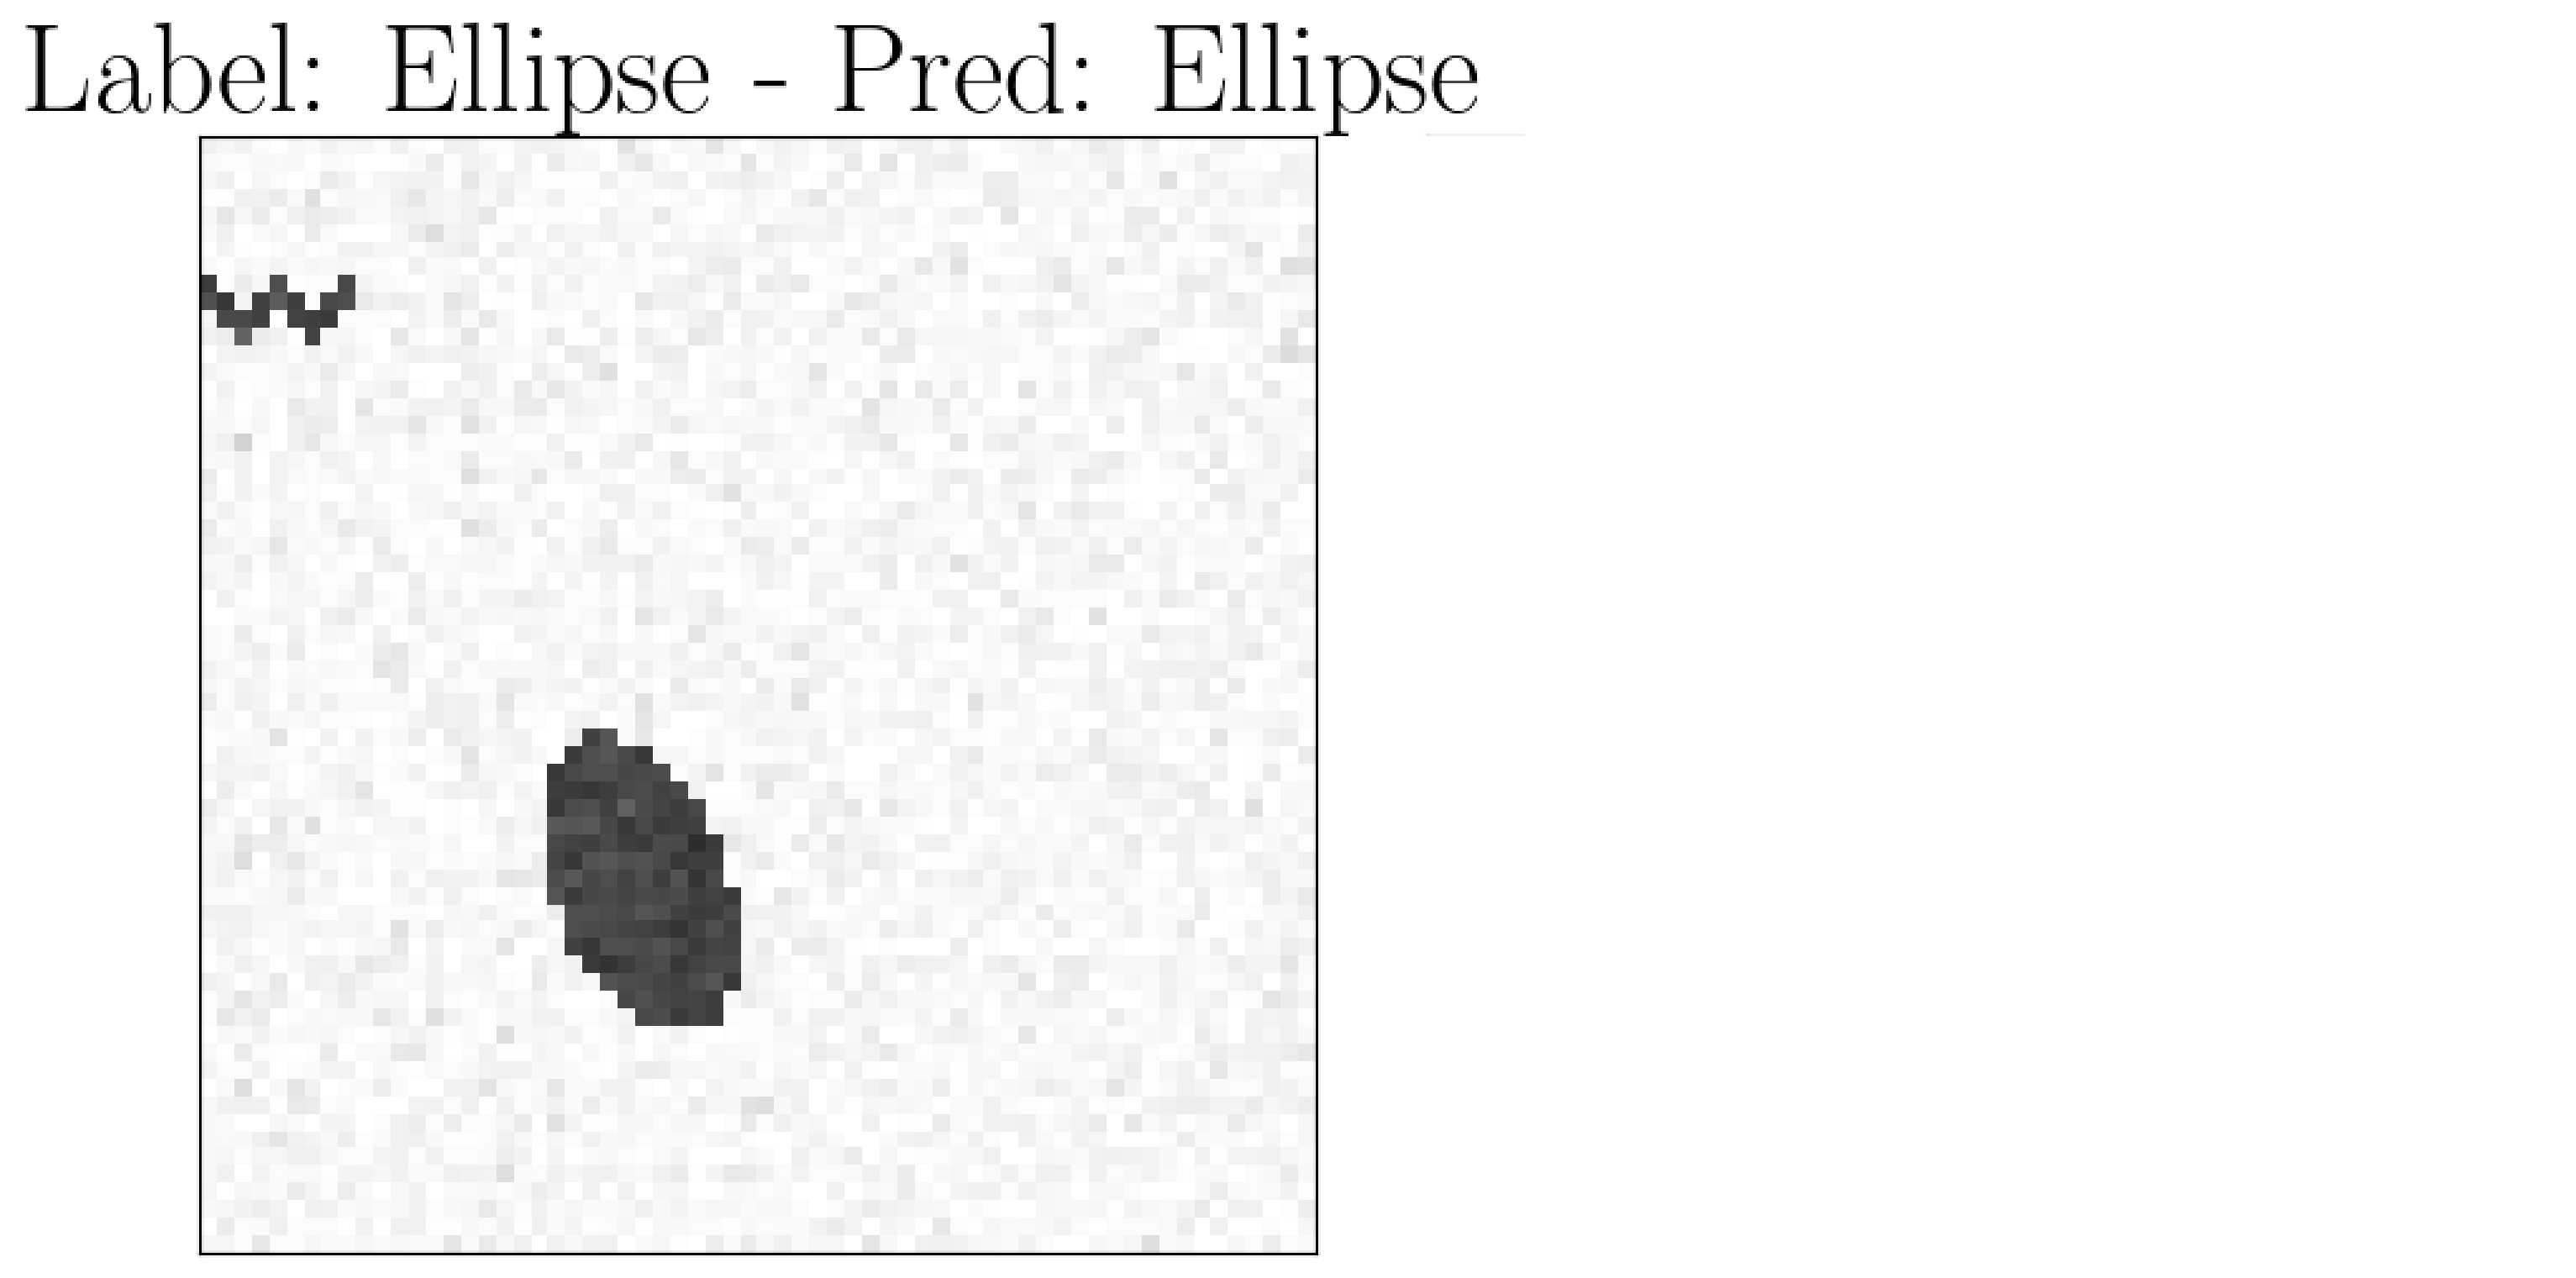
\includegraphics[width=\textwidth]{images/example_simple1.png}}{
                    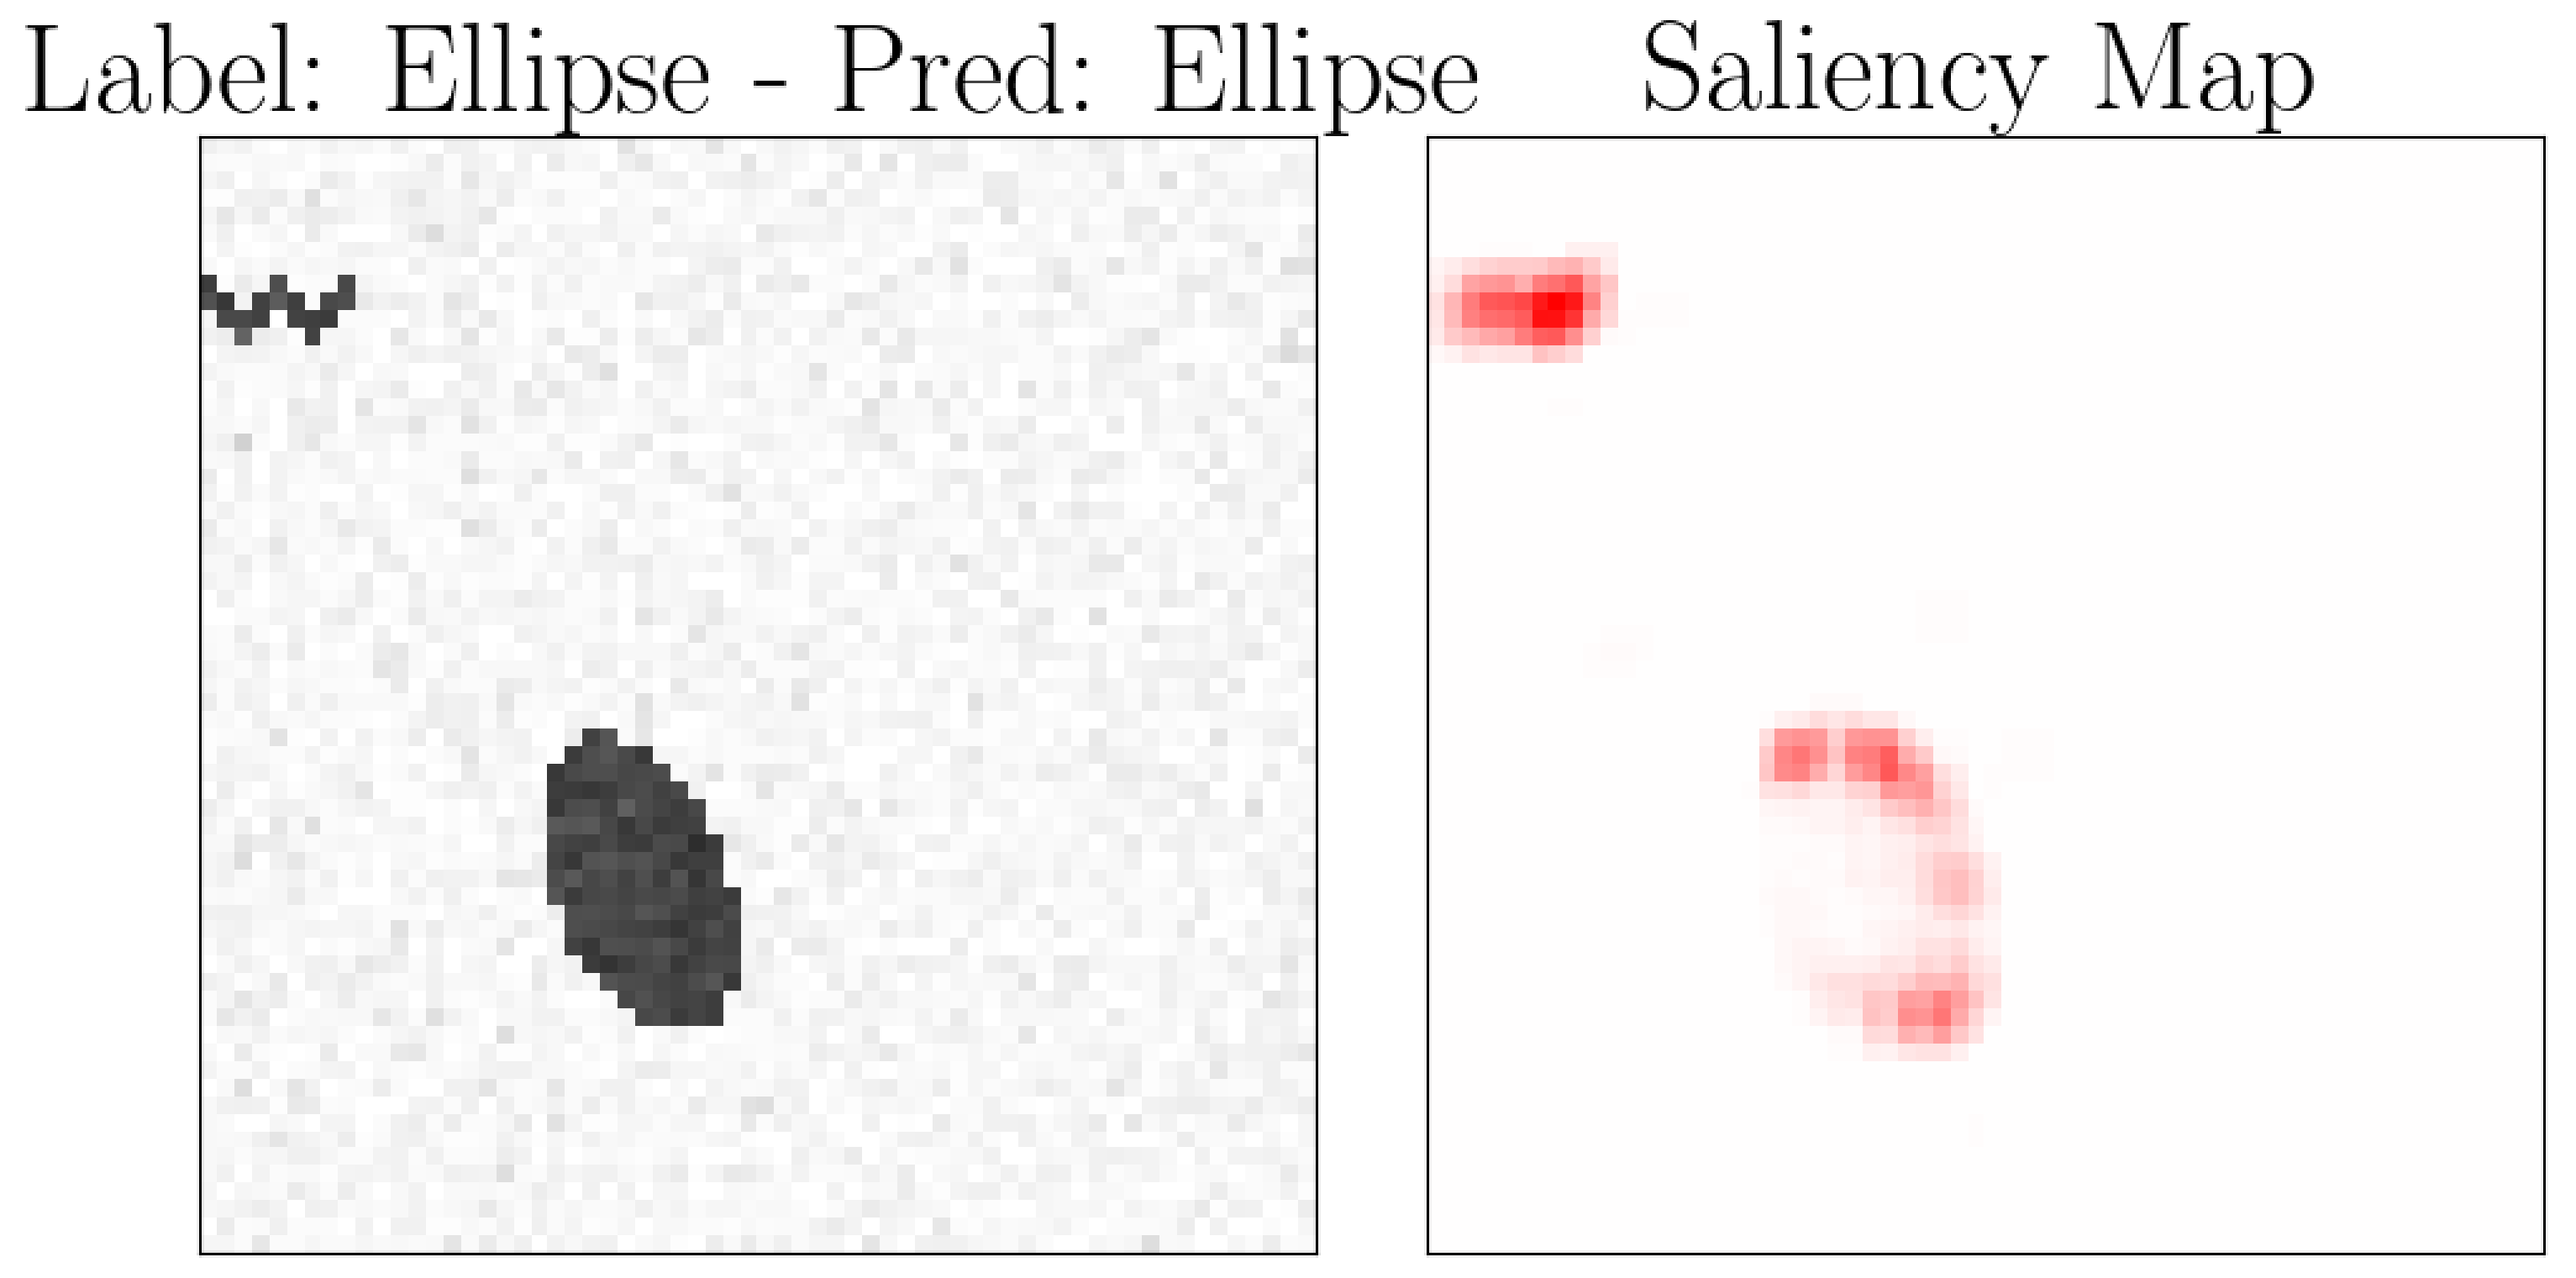
\includegraphics[width=\textwidth]{images/example_simple.png}}
            \end{figure}
        \end{column}
        \begin{column}{0.6\textwidth}
            \begin{itemize}
                \item Neural networks use unknown strategies to predict from data
                      \pause
                \item ``Clever-Hanses'' (spurious features) can be uncovered by explanation methods
                      \pause
                \item Concept-based methods claim finding relative feature importance
            \end{itemize}
        \end{column}
    \end{columns}
    \pause
    \vspace{0.4cm}
    \begin{block}{Research Question}
        Is the relative feature importance of a spurious feature explained by a concept-based method faithful to the model's true relative importance?
    \end{block}
\end{frame}

%----------------------------------------------------------------------------------------
\subsection{Concept Relevance Propagation (CRP)}
\begin{frame}[t]{Concept Relevance Propagation (CRP \cite{Achtibat2023})}
    \vspace{-0.5cm}
    \begin{itemize}
        \item Framework built on top of modified Layerwise Relevance Propagation (LRP \cite{Bach2015} \footpartcite{Bach2015})
        \item Conditionally masks neurons to obtain concept specific relevances and heatmaps
    \end{itemize}
    \vspace{-0.5cm}
    \begin{figure}
        \centering
        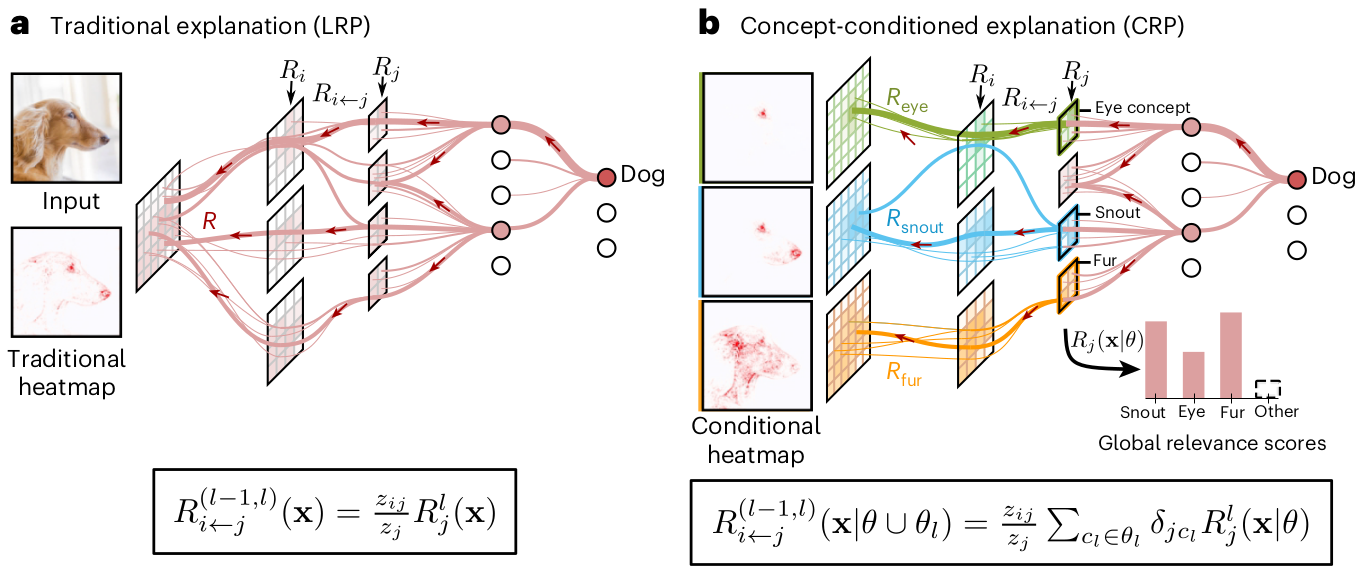
\includegraphics[width=0.7\textwidth]{images/crp_vs_lrp_from_paper.png}
    \end{figure}
    \vspace{-0.5cm}
    \footpartcite{Achtibat2023}
\end{frame}

%----------------------------------------------------------------------------------------
\begin{frame}[t]{Concept-Conditional Heatmaps and Reference Sets}
    \begin{figure}
        \begin{overlayarea}{\textwidth}{\textheight}
            \only<1>{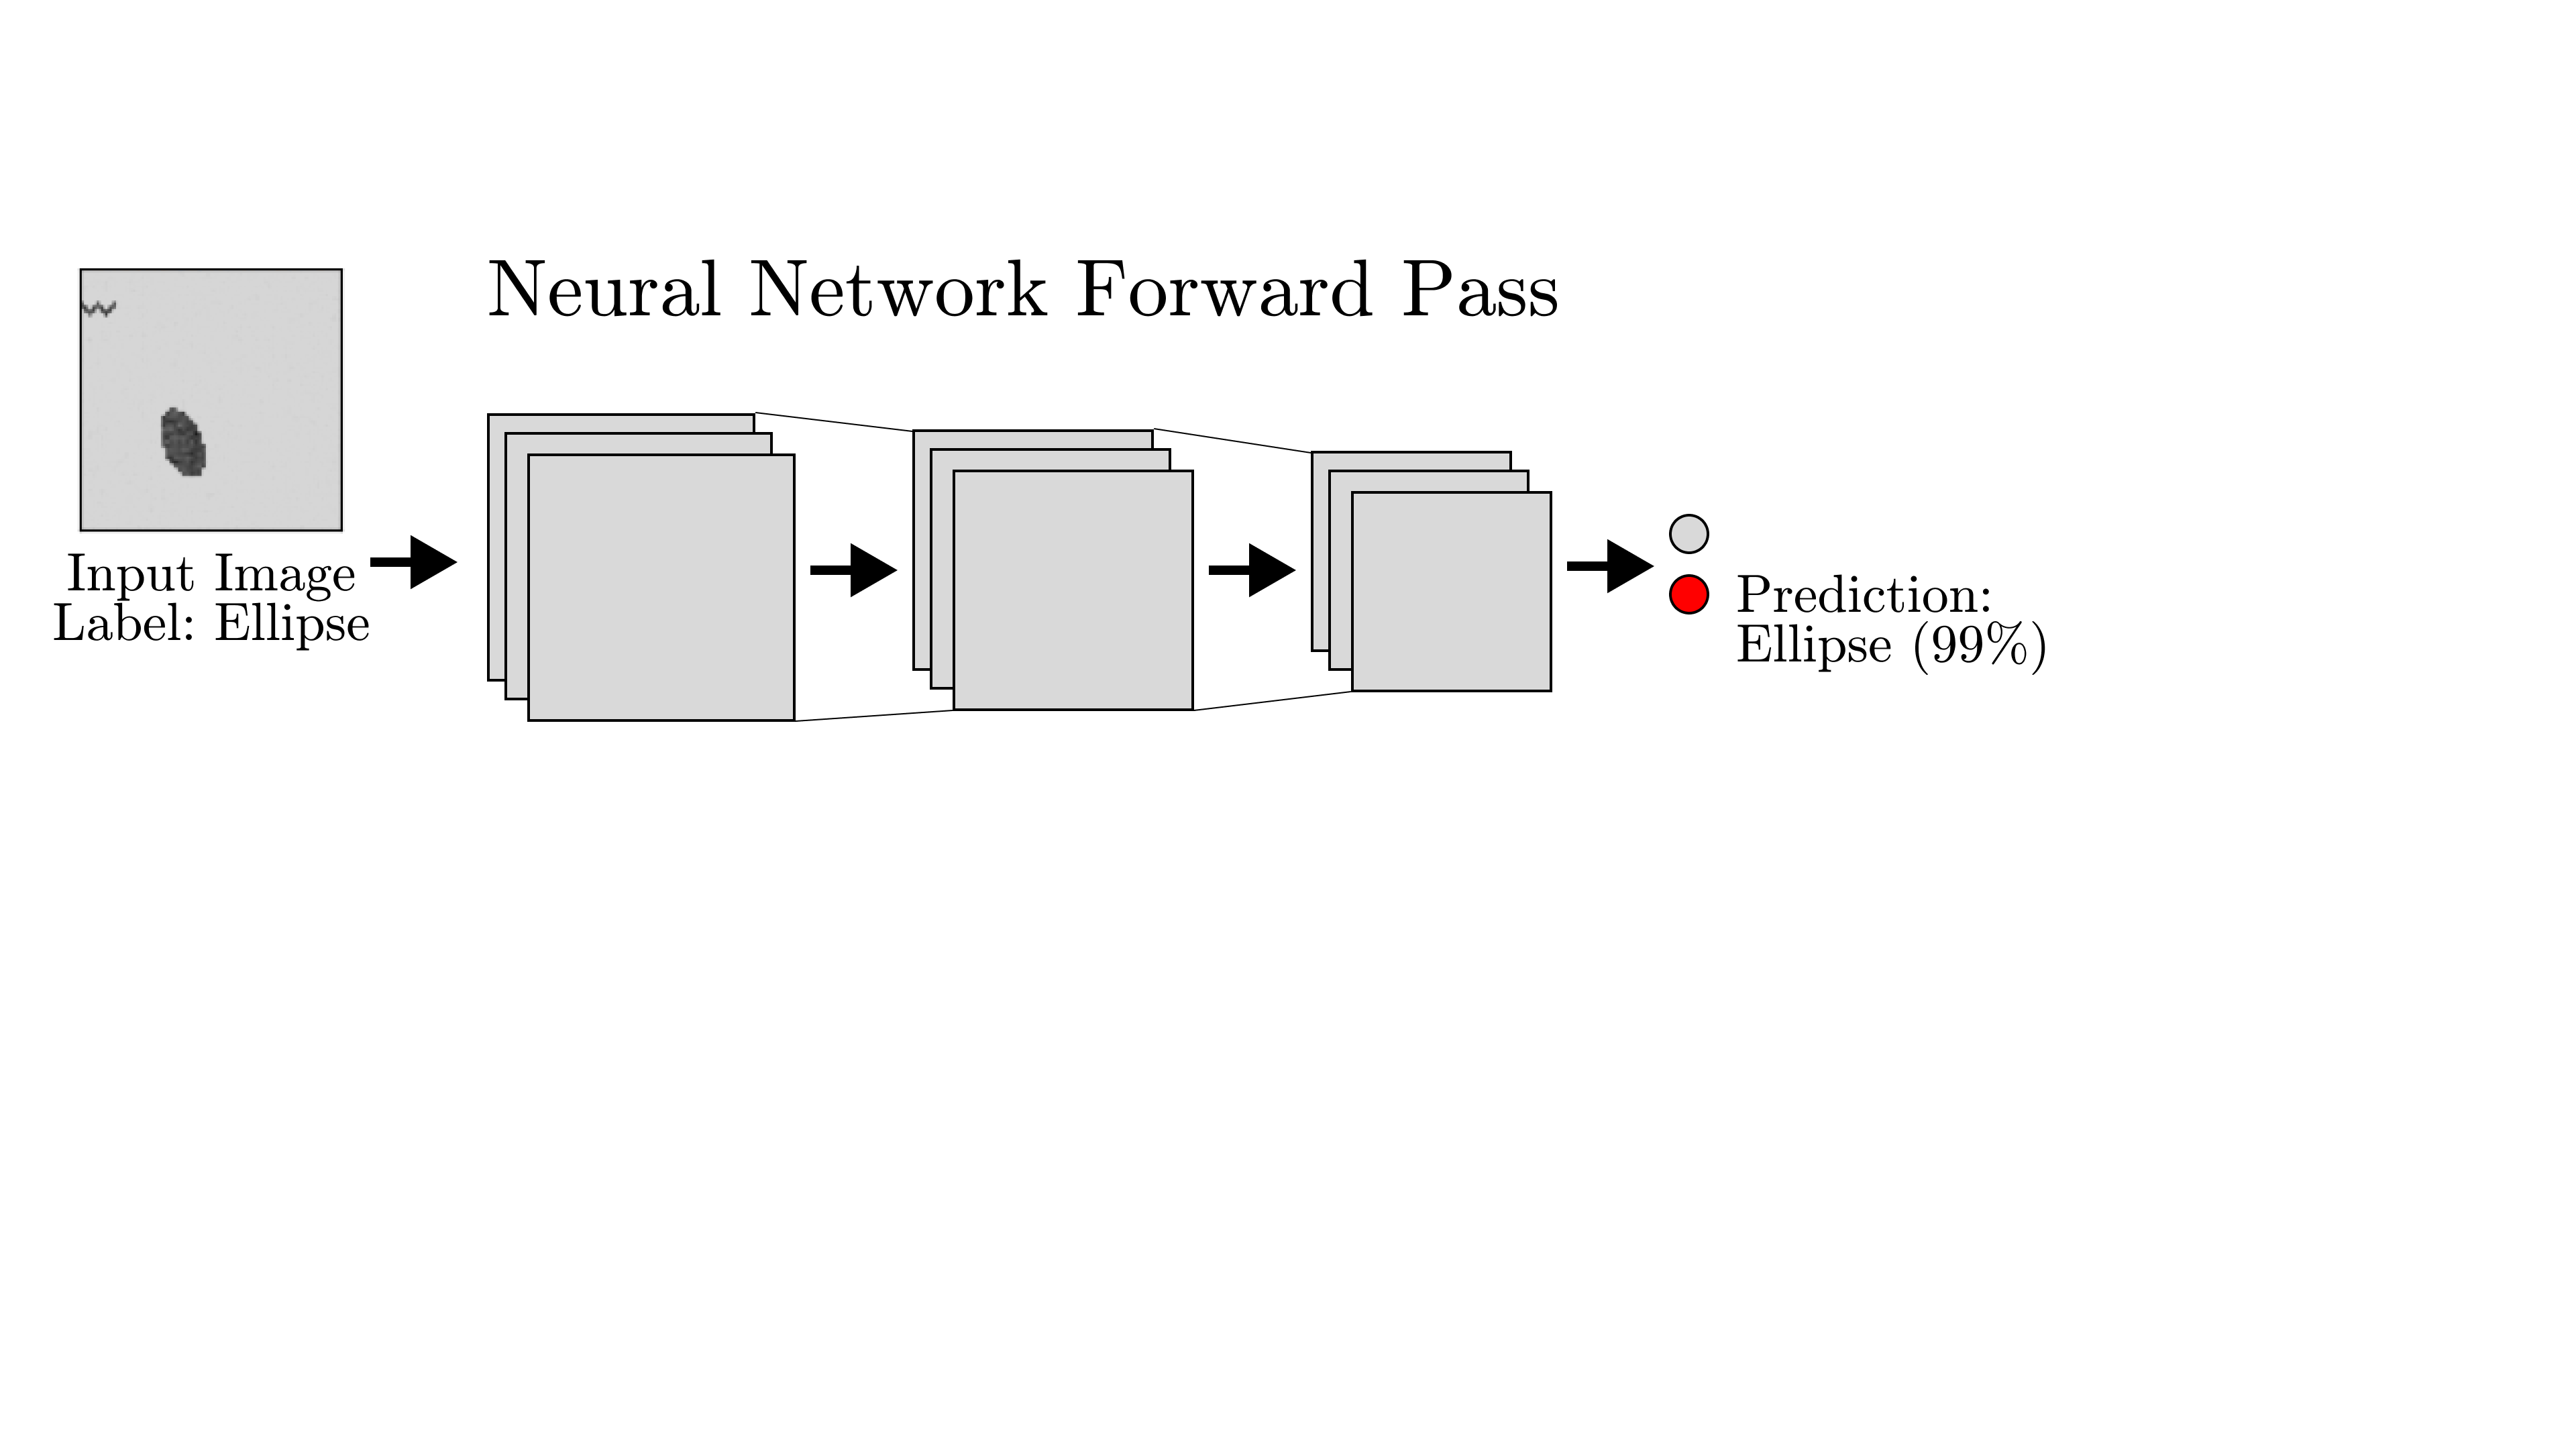
\includegraphics[width=0.9\textwidth]{images/crp_explain_0.png}}
            \only<2>{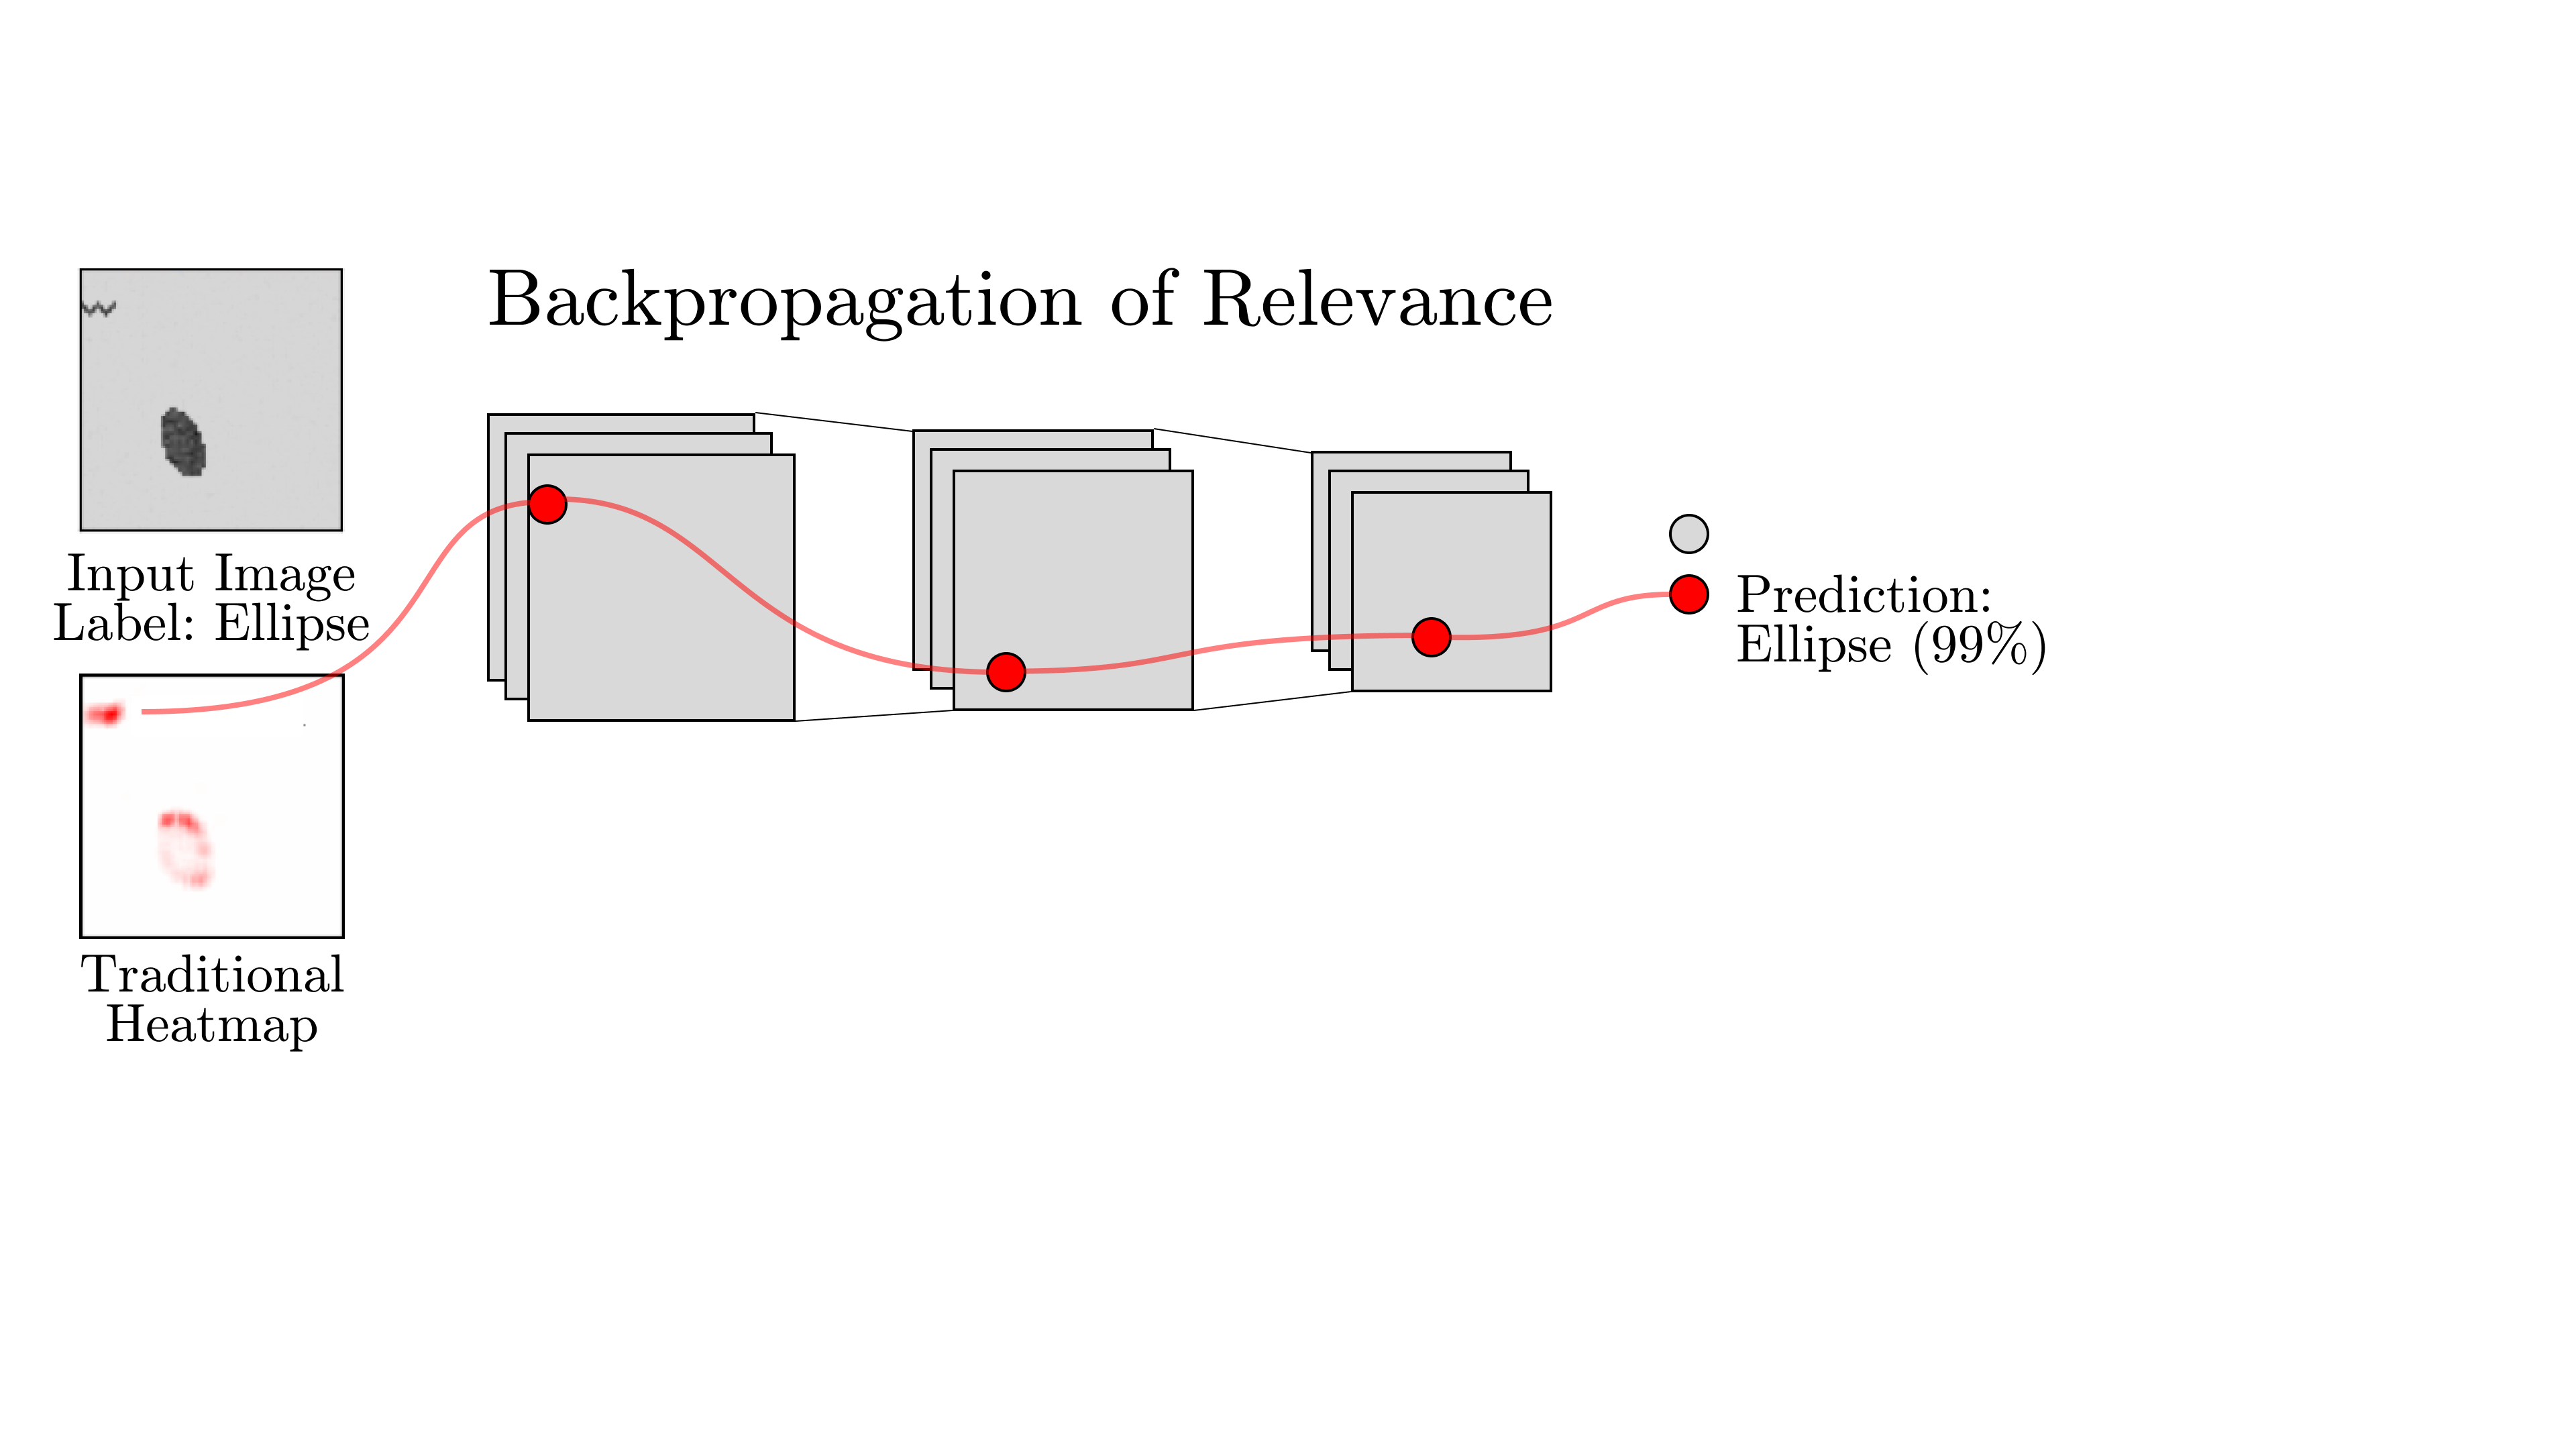
\includegraphics[width=0.9\textwidth]{images/crp_explain_1.png}}
            \only<3>{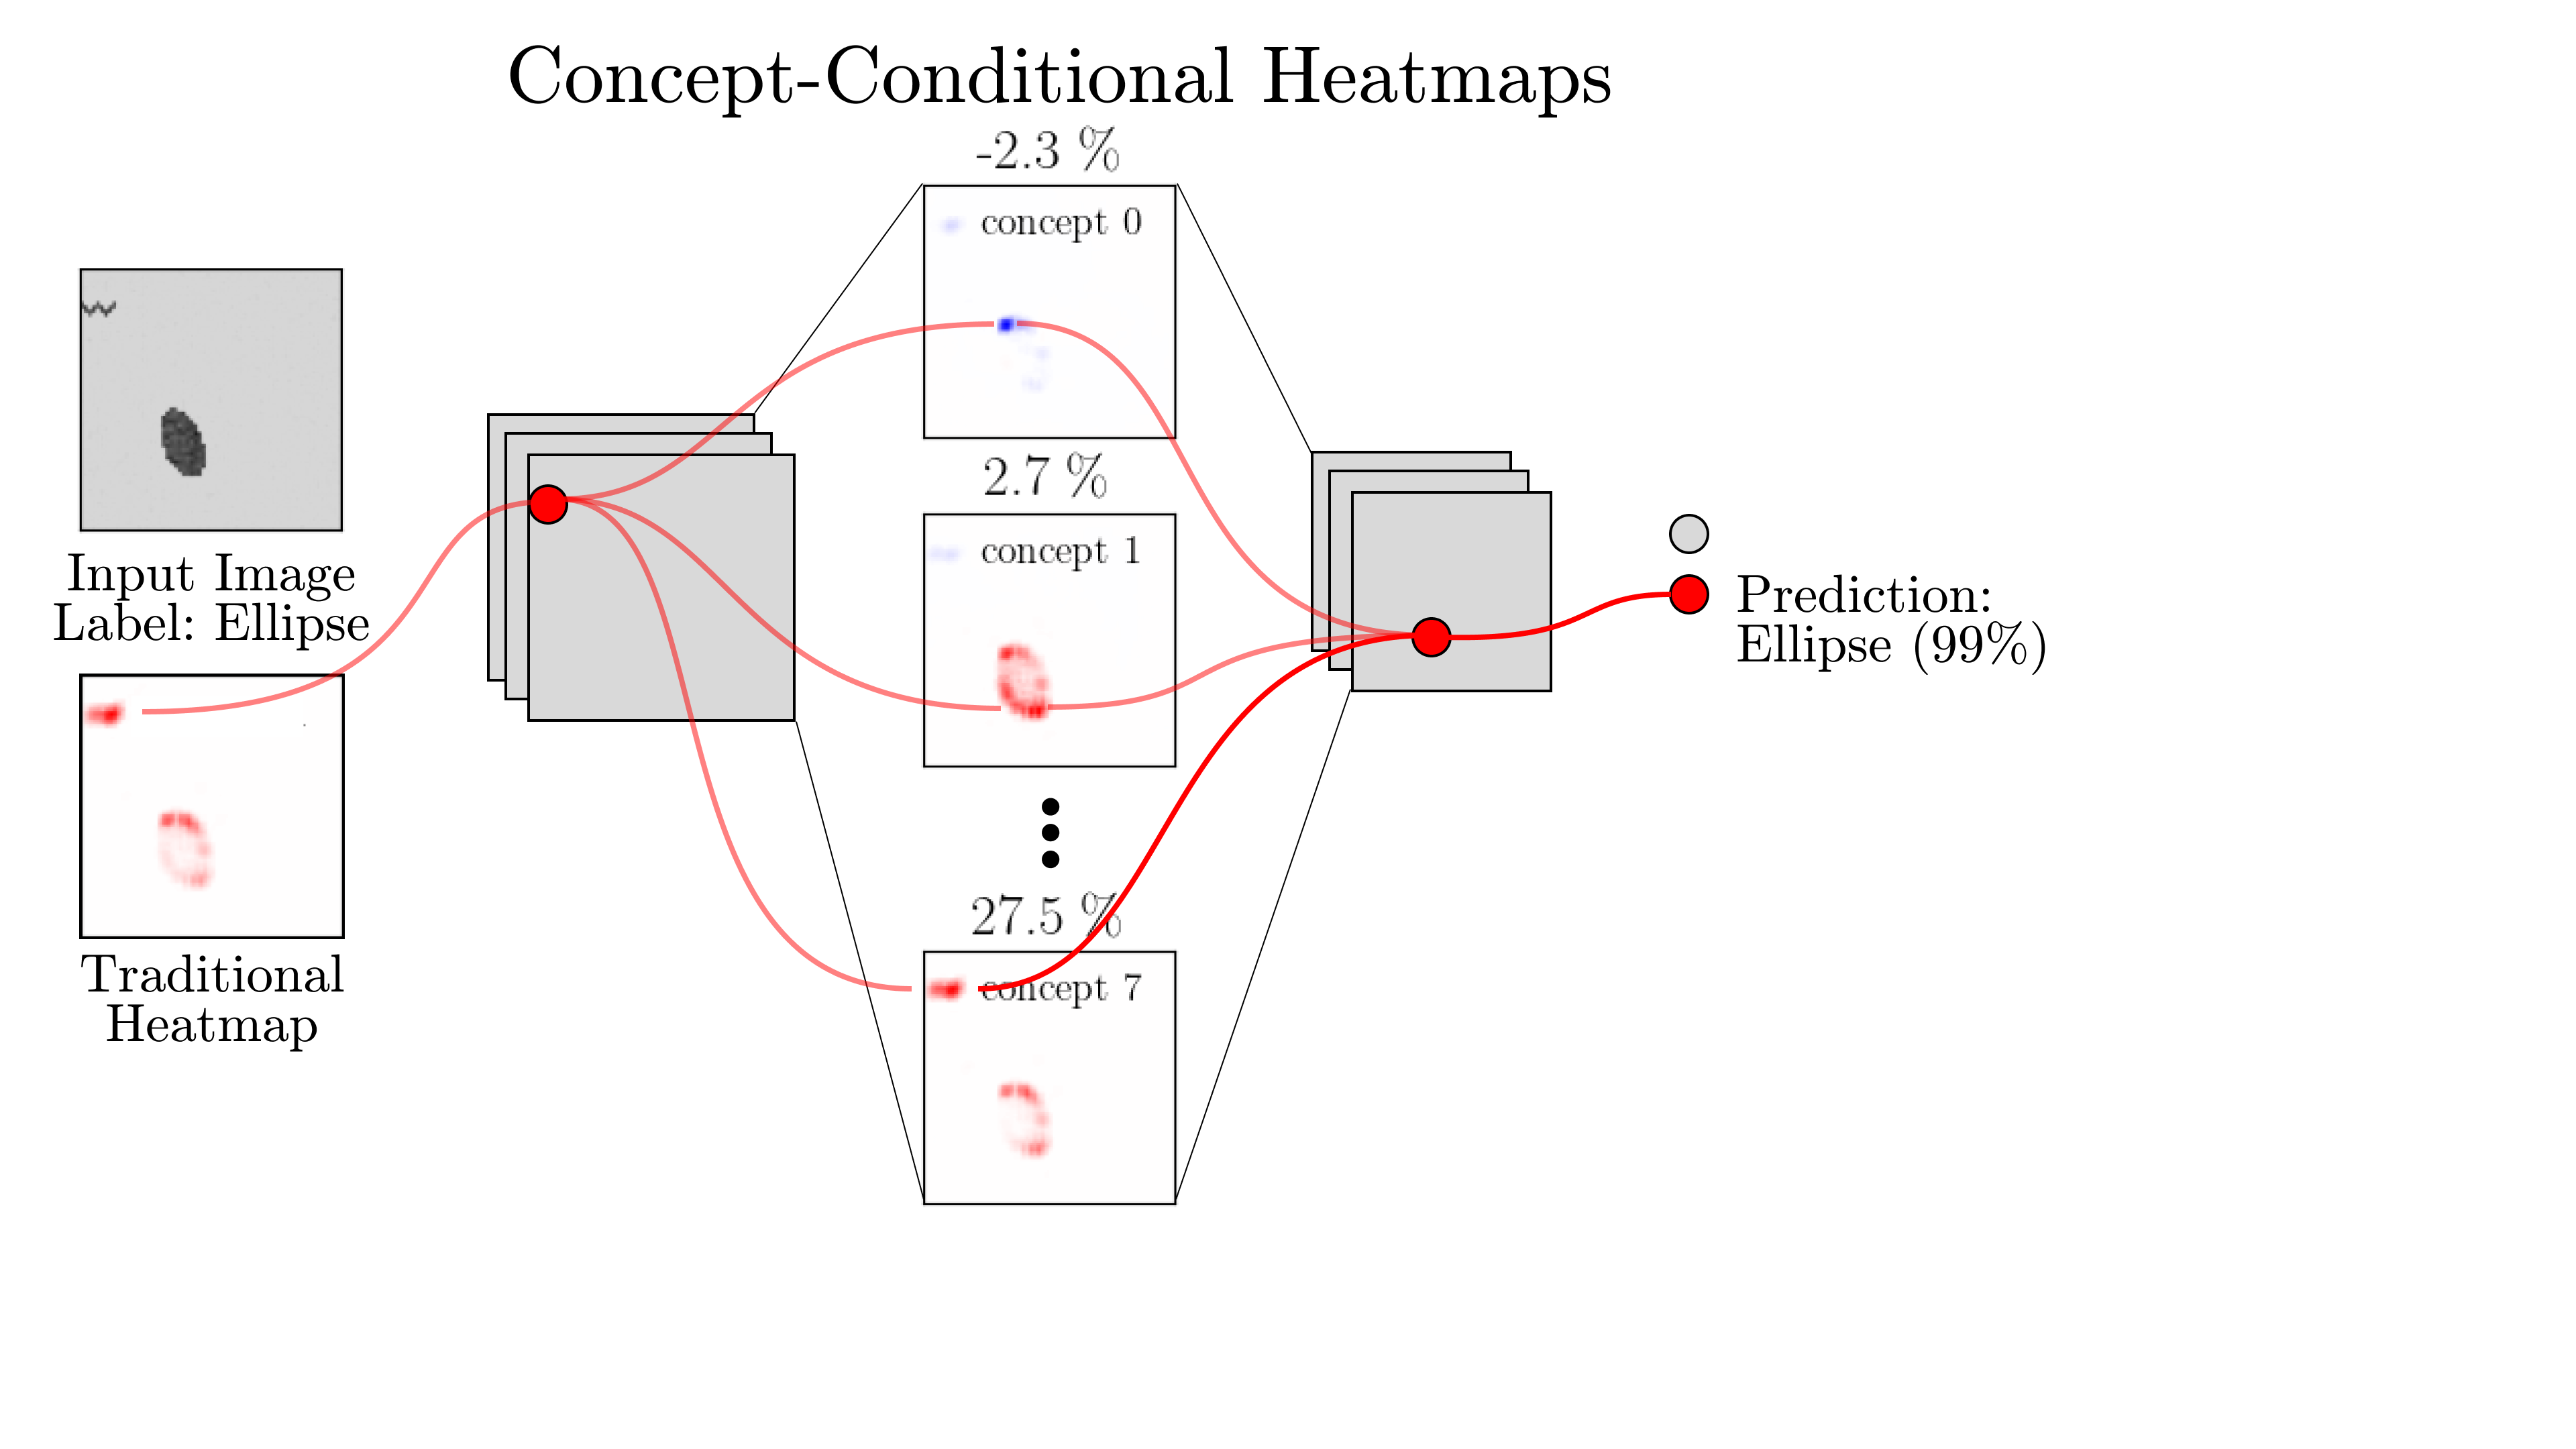
\includegraphics[width=0.9\textwidth]{images/crp_explain_2.png}}
            \only<4>{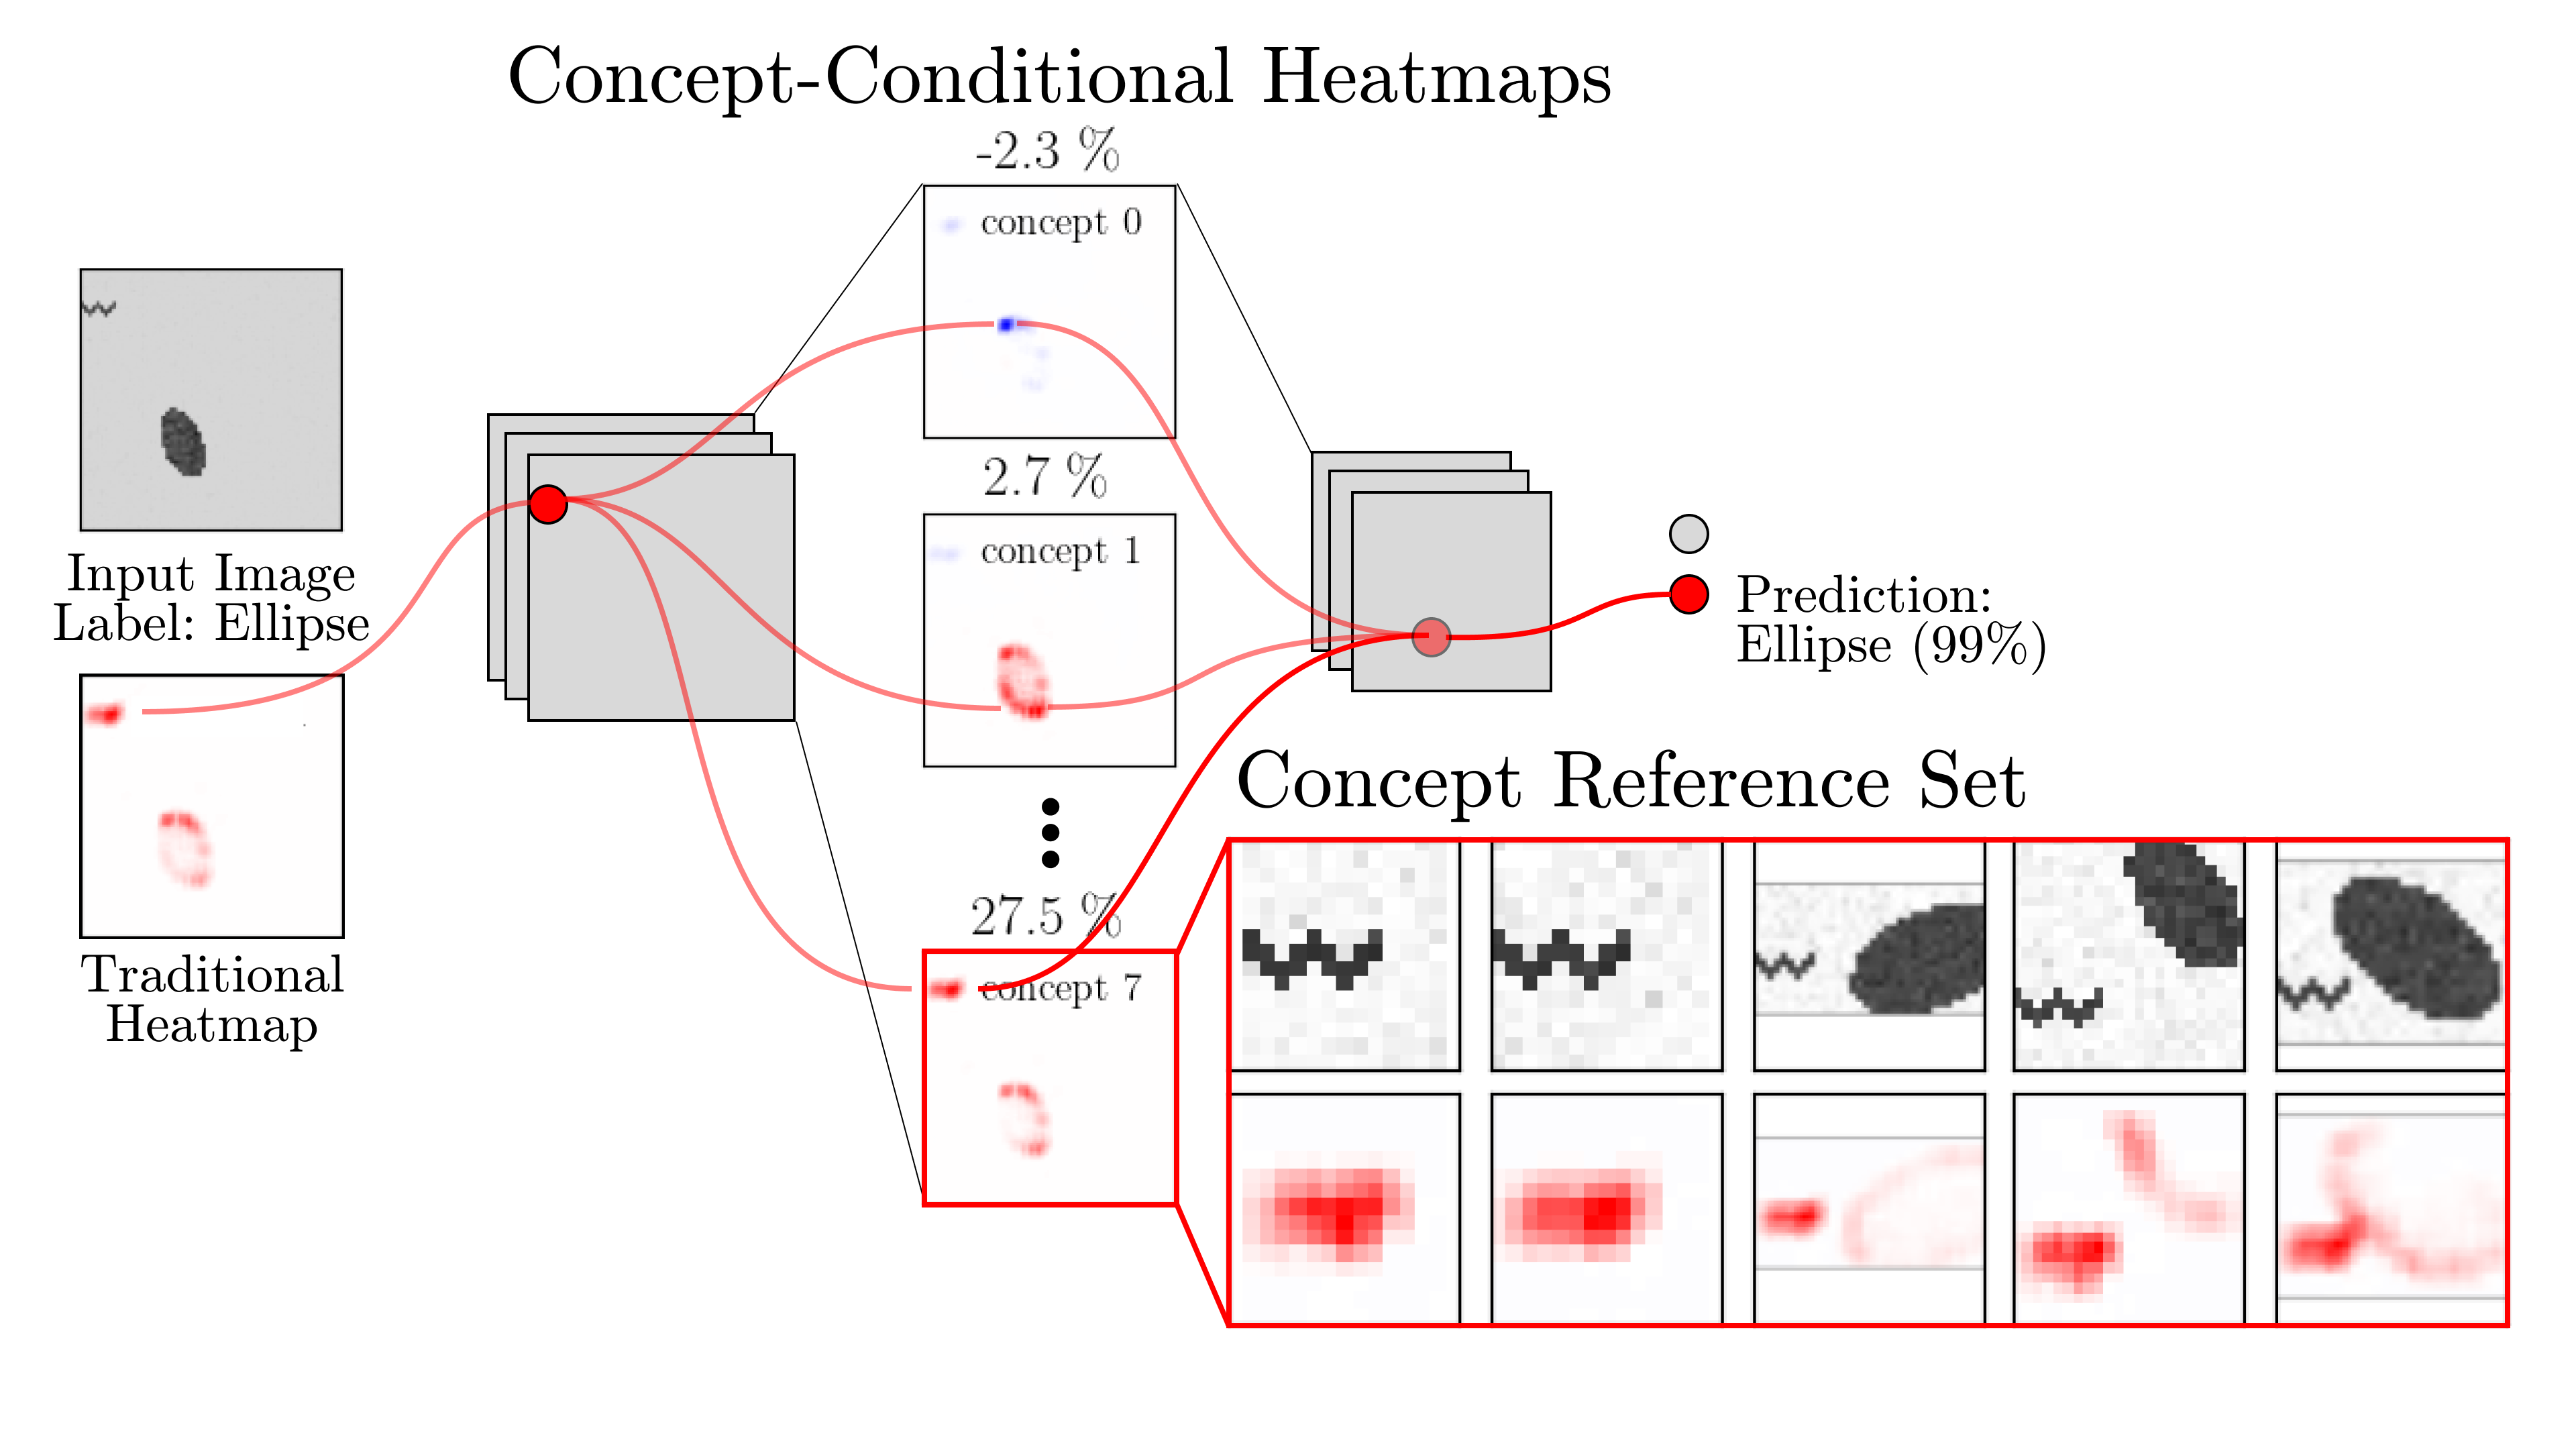
\includegraphics[width=0.9\textwidth]{images/crp_explain_3.png}}
        \end{overlayarea}
    \end{figure}
\end{frame}

%----------------------------------------------------------------------------------------
% now we have seen how CRP can uncover the strategies a model has maybe wrongly learned
% but have we really seen that? looking at these explanations, while they are visually appealing, is just anecdotal evidence, it was also a very simple dataset
% in real datasets, especially image datasets, we don't always know what the "correct" strategy is, because even we humans don't understand the true causal relationships between features in an image
% to evaluate CRP systematically, and especially the *relative* feature importance, we therefore need a dataset, where we know all the exact relationships
% the causality framework gives us the tools to generate data with known causal relationships and distributions
% even though we use a very reduced and simple dataset, it can theoretically be applied to many 
\subsection{Causality Framework}
\begin{frame}{Causal Evaluation of CRP}
    \begin{columns}
        \begin{column}{0.3\textwidth}
            \begin{figure}
                \centering
                \tikzset{%
                    normal/.style={
                            draw,
                            minimum height=6mm,
                            minimum width=7mm,
                            inner sep=2pt,
                            align=center,
                            scale=0.8
                        },
                }
                %\begin{mdframed}[backgroundcolor=graybg]
                \begin{tikzpicture}[scale=1.0]
                    \node [normal]  (a) at (0,3) {
                        \alt<1-2>{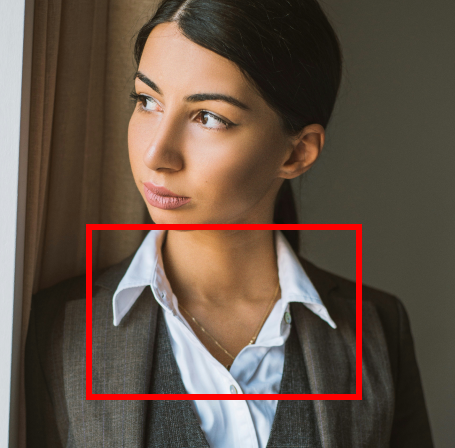
\includegraphics[width=0.3\textwidth]{images/woman_suit_collar.jpg}}
                        {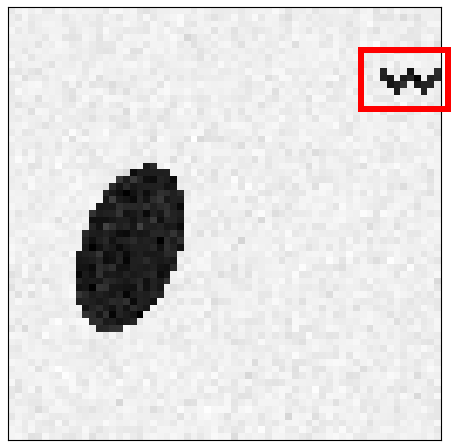
\includegraphics[width=0.3\textwidth]{images/spurious_feature.png}}
                        \\ Spurious \\ Feature};
                    \node [normal]  (b) at (0,0) {
                        \alt<1-2>{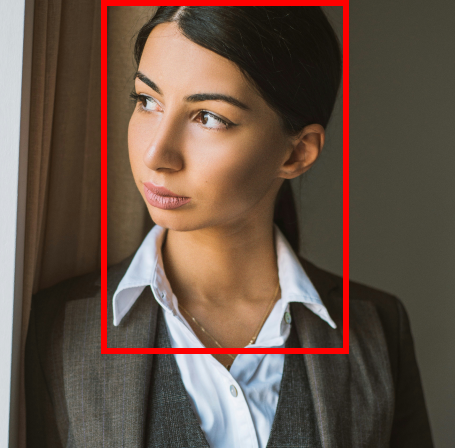
\includegraphics[width=0.3\textwidth]{images/woman_suit_face.jpg}}
                        {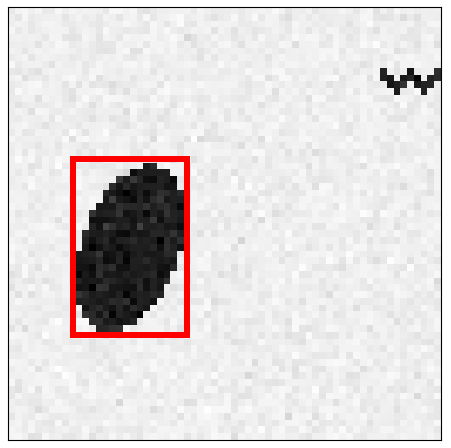
\includegraphics[width=0.3\textwidth]{images/core_feature.png}}
                        \\ Core \\ Feature};
                    \node [normal]  (c) at (2,1.5) {
                        \alt<1-2>{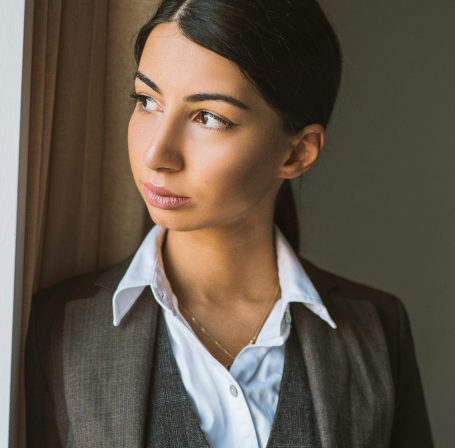
\includegraphics[width=0.3\textwidth]{images/woman_suit.jpg}}
                        {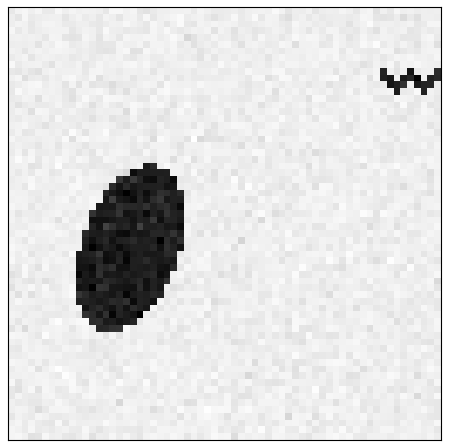
\includegraphics[width=0.3\textwidth]{images/cs_image.png}}
                        \\ Image};


                    \alt<1-2>{\node []  (x) at (0,1.5) {?};
                        \node []  (y) at (1,2.5) {?};
                        \node []  (y) at (1,0.5) {?};}{

                        \draw[->] (a) -- (c);
                        \draw[->] (b) -- (c);
                        \draw[<->] (b) -- (a);
                    }
                \end{tikzpicture}
            \end{figure}
        \end{column}
        \begin{column}{0.7\textwidth}
            \begin{itemize}
                \item In real datasets anecdotal identification of spurious and core features, not coherence to model \cite{Nauta2023}
                      \pause
                \item Evaluating feature importance requires knowing ground-truth data distribution and ground-truth strategy of model\pause
                \item Causality framework defines how data is generated and enables measuring true model strategy
            \end{itemize}
        \end{column}
    \end{columns}
    \footnote[1]{Photo by Ana Itonishvili on Unsplash}
    \footpartcite{Nauta2023}
\end{frame}

\begin{frame}{Causality Framework}
    \begin{columns}[t]
        \begin{column}{.6\textwidth}
            \textbf{Structural Causal Model (SCM)}
            \begin{itemize}
                \item Observable variables $V$
                \item Unobserved variables $U$,  probability dist. $P_u$
                \item Structural assignments $f_x({Pa}_{x}, u_x)$ between a variable $X$ and its parents ${Pa}_{x} \in (V \setminus \{X\}) \cup U$
            \end{itemize}
        \end{column}
        \begin{column}{.4\textwidth}
            \textbf{Causal Graph}
            \begin{figure}
                \centering
                \tikzset{%
                    neuron/.style={
                            ellipse,
                            draw,
                        },
                    arrows={[scale=1.2]}
                }
                %\begin{mdframed}[backgroundcolor=graybg]
                \begin{tikzpicture}[scale=0.9]
                    % generating model:
                    \node [neuron]  (a) at (3,2) {$Z$};
                    \node [neuron, dashed]  (b) at (0,2) {$U$};
                    \only<1>{\node [neuron]  (c) at (0,0) {$X$};}
                    \only<2>{\node [neuron, fill=teal!10]  (c) at (0,0) {$X$};}
                    \node [neuron]  (d) at (3,0) {$Y$};


                    \draw[->] (c) -- (d);
                    \only<1>{\draw[->] (a) -- (c);
                        \draw[->] (b) -- (c);}
                \end{tikzpicture}
            \end{figure}
        \end{column}
    \end{columns}
    \pause
    Do-Calculus by Judea Pearl (\cite{Pearl2009} \footpartcite{Pearl2009}): Estimate Causal Effects\\
    Average Causal Effect of Intervention on X:
    \begin{align*}
        \displaystyle \mathrm{ACE} : & = \mathbb{E} [ Y \ | \ do(X=1) ] - \mathbb{E} [ Y \ | \ do(X=0) ] \\
        %& = \mathbb{E}_Z \left\{ \frac{\partial}{\partial x} [ Y \ | \ X=x, Z=z ] \right\}
    \end{align*}
\end{frame}
%----------------------------------------------------------------------------------------

\section
 [Methods]{Methods}
%----------------------------------------------------------------------------------------
\begin{frame}{Strategy} %<presentation:0>[noframenumbering]
    \begin{figure}
        \centering
        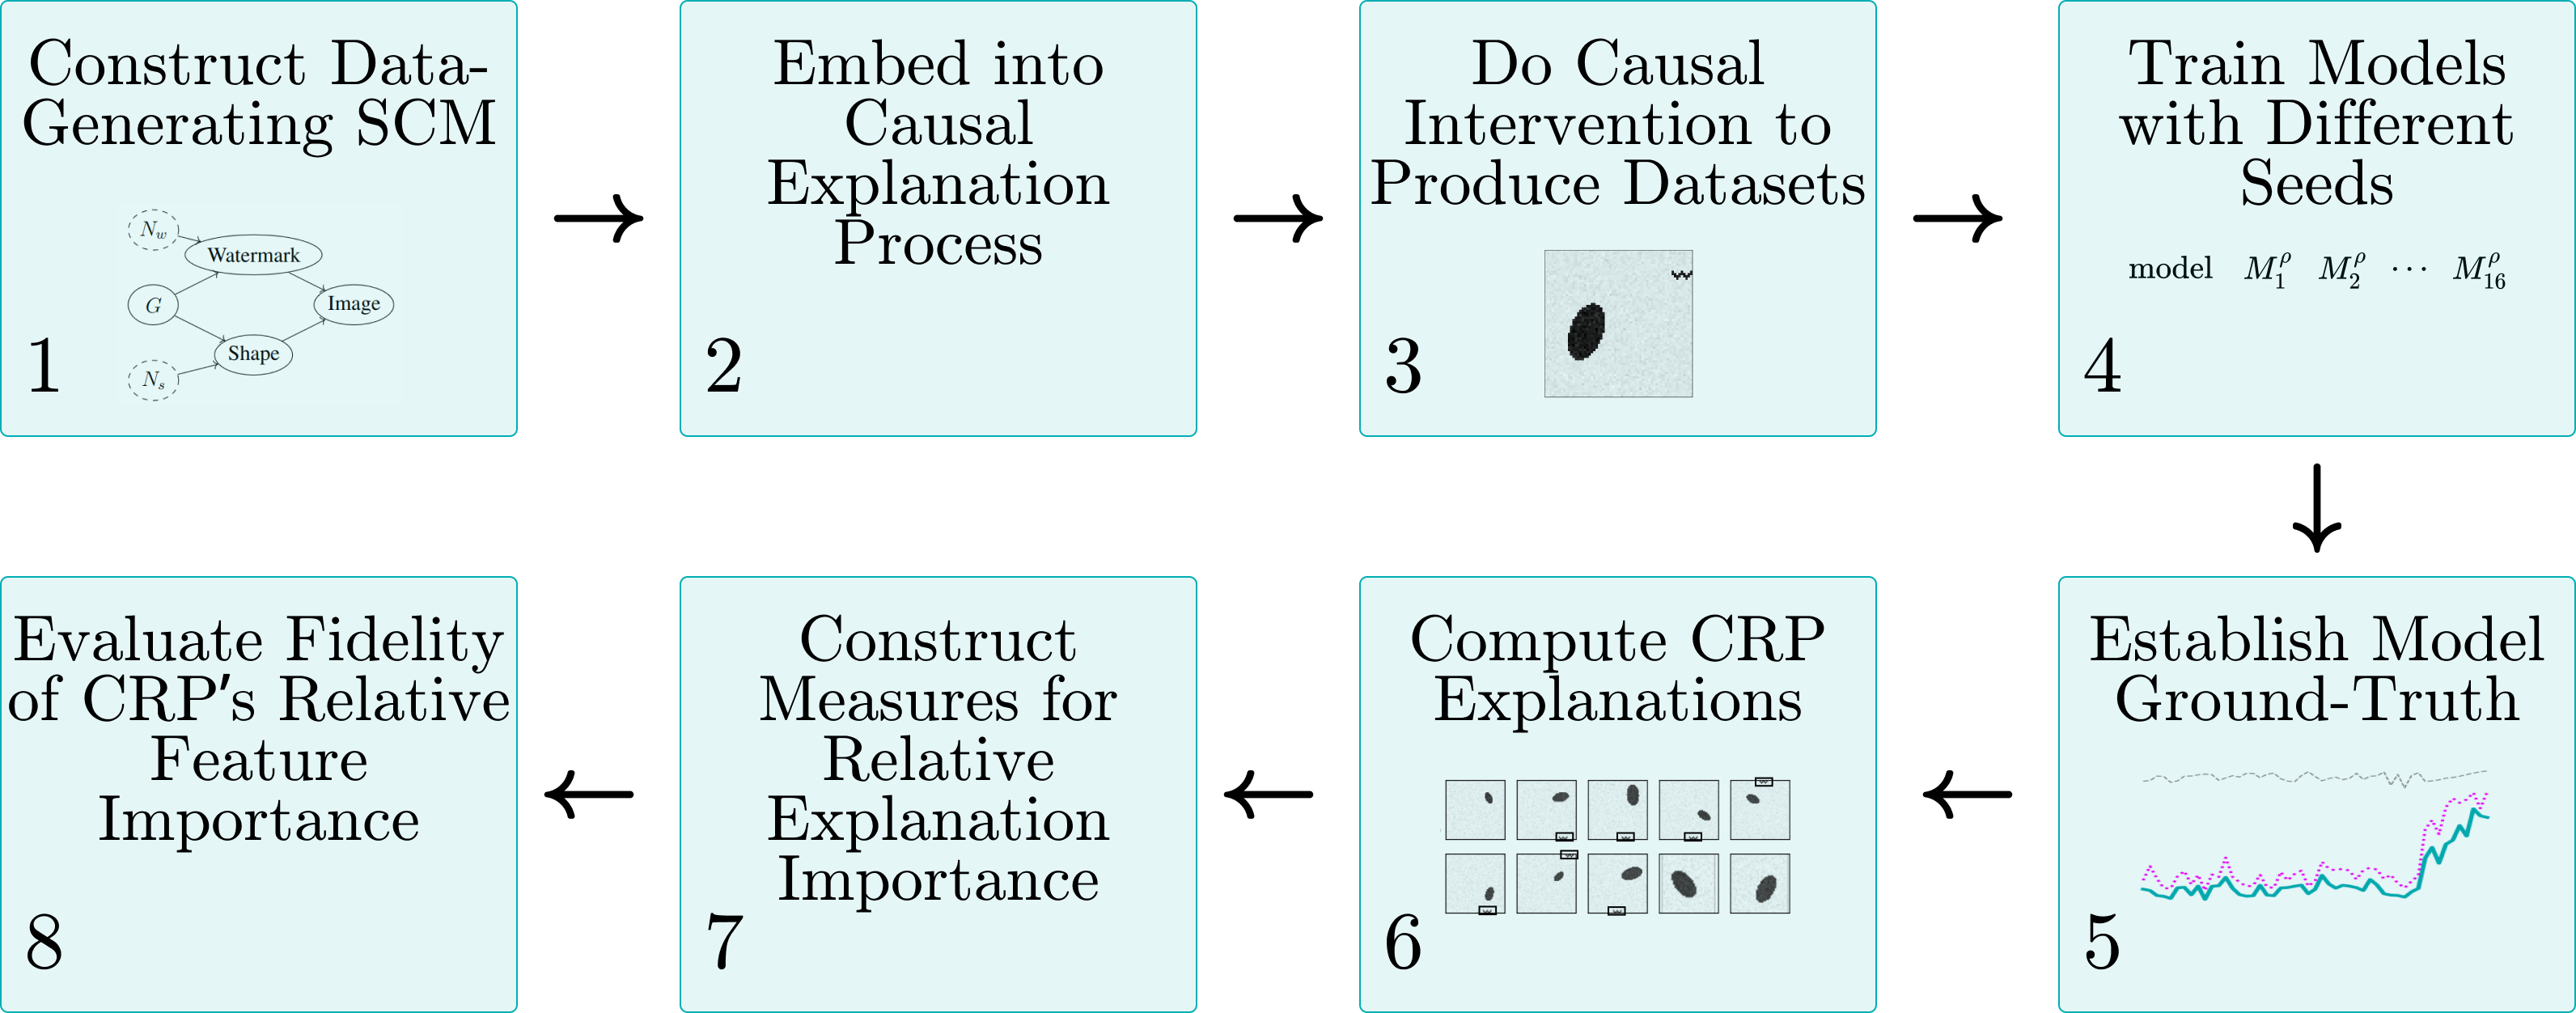
\includegraphics[width=\textwidth]{images/strategy1.png}
    \end{figure}
\end{frame}
%----------------------------------------------------------------------------------------
\subsection{Causal Model}
\begin{frame}[t]{Causal Data Generating Model}
    \begin{columns}[t]
        \begin{column}{.4\textwidth}
            \vspace{-0.5cm}
            \begin{align*}
                S & :=(\textcolor{teal}{\rho} * G + (1-\textcolor{teal}{\rho})\cdot \mathcal{N}_s) \geq \tfrac{1}{2} \\
                Z & := \mathcal{U}_{z^4}                                                                             \\
                G & :=\mathcal{N}_g                                                                                  \\
                W & :=(\textcolor{teal}{\rho} * G + (1-\textcolor{teal}{\rho})\cdot \mathcal{N}_w) \geq \tfrac{1}{2} \\
                X & := W + f_{image}(S, Z) + \mathcal{N}_{x}                                                         \\
            \end{align*}
            \vspace{-1.7cm}
            \begin{overlayarea}{\textwidth}{0.34\textheight}
                \begin{figure}
                    \visible<3>{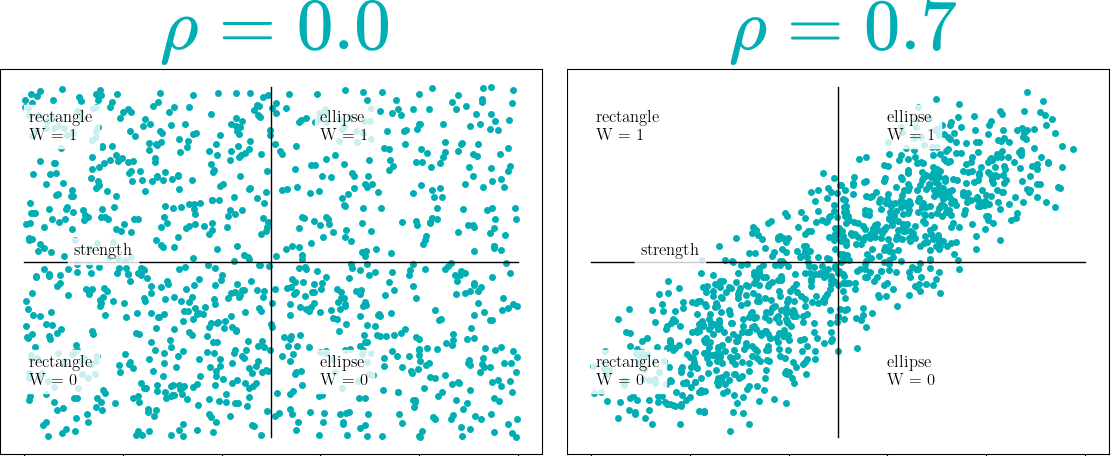
\includegraphics[width=\textwidth]{images/distribution.png}}
                    \label{fig:distribution}
                \end{figure}
            \end{overlayarea}
        \end{column}
        \begin{column}{.6\textwidth}
            \begin{figure}
                \centering
                \tikzset{%
                    neuron/.style={
                            ellipse,
                            draw,
                            minimum height=5mm,
                            minimum width=7mm,
                            inner sep=1pt,
                            align=center,
                            scale=0.6
                        },
                }
                \begin{tikzpicture}[scale=0.8]
                    % generating model:
                    \node [neuron, dashed]  (nw) at (0,4) {Watermark Noise \\$N_w$};
                    \node [neuron, dashed]  (g) at (0,2) {Generator Noise\\$G$};

                    \node [neuron]  (w) at (2.5,3) {Watermark \\$W$};
                    \visible<2>{\node [neuron, fill=teal!10]  (w) at (2.5,3) {Watermark \\$W$};}
                    \visible<2-3>{
                        \node[inner sep=0pt] (spurious) at (2.5,4.5)
                        {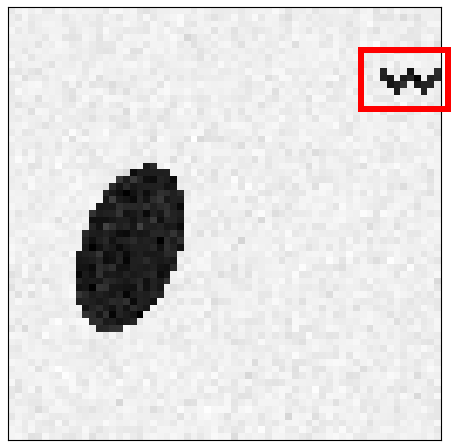
\includegraphics[width=0.14\textwidth]{images/spurious_feature.png}};}

                    \node [neuron]  (s) at (2.5,1) {Shape \\$S$};
                    \visible<1>{\node [neuron, fill=teal!10]  (s) at (2.5,1) {Shape \\$S$};}
                    \visible<1-3>{
                        \node[inner sep=0pt] (spurious) at (2.5,-0.5)
                        {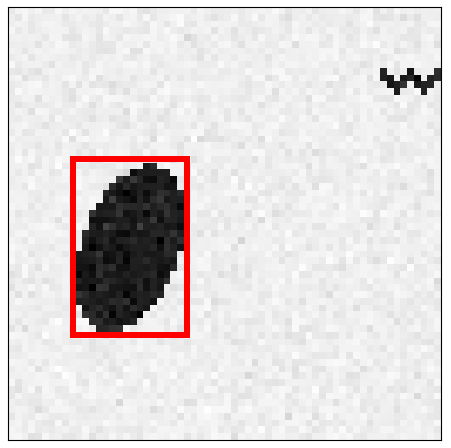
\includegraphics[width=0.14\textwidth]{images/core_feature.png}};}

                    \node [neuron, dashed]  (ns) at (0,0) {Shape Noise \\$N_s$};
                    \node [neuron]  (x) at (5,2) {Image \\$X$};
                    \visible<1>{\node [neuron, fill=teal!10]  (xx) at (5,2) {Image \\$X$};}
                    \node [neuron]  (z) at (5,0) {Other Factors \\$Z$};
                    \node [neuron, dashed]  (nx) at (5,4) {Image Noise \\$N_x$};

                    \draw[->] (nw) -- (w);
                    \draw[->] (g) -- (w);
                    \draw[->] (g) -- (s);
                    \draw[->] (w) -- (x);
                    \draw[->] (ns) -- (s);
                    \draw[->] (s) -- (x);
                    \draw[->] (z) -- (x);
                    \draw[->] (nx) -- (x);
                \end{tikzpicture}
            \end{figure}
        \end{column}
    \end{columns}
    \pause
    Watermark W and Shape S are confounded by Generator G through a coupling ratio $\textcolor{teal}{\rho}$
\end{frame}
%----------------------------------------------------------------------------------------

\begin{frame}[t]{Causal Explanation Generation Process}
    \begin{figure}[t!]
        \centering
        \tikzset{%
            neuron/.style={
                    ellipse,
                    draw,
                    minimum height=8mm,
                },
            arrows={[scale=1.2]}
        }
        %\begin{mdframed}[backgroundcolor=graybg]
        \begin{tikzpicture}[scale=0.9]
            % generating model:
            \node [neuron, fill=teal!10]  (r) at (0,4) {$\rho$};
            \node [neuron, fill=teal!10]  (rs) at (5,3) {seed};
            \node [neuron]  (scm) at (3,4) {DATA};
            \node [neuron]  (w) at (7,4) {model};
            \node [neuron]  (x) at (7,2) {$X$};
            \node [neuron]  (p) at (9,3) {$Y$};
            \node [neuron]  (e) at (11,2) {$E$};

            \draw[->] (r) -- (scm);
            \draw[->] (scm) -- (w);
            \draw[->] (rs) -- (w);
            \draw[->] (w) -- (p);
            \draw[->] (x) -- (p);
            \draw[->, bend left=40] (w) to (e);
            \draw[->, bend right=20] (x) to (e);
            \draw[->] (p) -- (e);
        \end{tikzpicture}\\
        \centering{inspired by Karimi et al. \cite{Karimi2023} \footpartcite{Karimi2023}}
    \end{figure}
    \textcolor{teal}{$\rho$}: coupling ratio,  \textcolor{teal}{seed}: random initialization,\\
    DATA: Training Dataset, model: state after training,\\
    $Y$: Prediction, $X$: Input Image, $E$: Explanation (Importance)
\end{frame}
%----------------------------------------------------------------------------------------
\subsection{Benchmark Datasets}
\begin{frame}{Benchmark Datasets}
    \centering
    \begin{enumerate}\addtocounter{enumi}{-1}
        \item Original \textit{dSprites} dataset \cite{dsprites17} \footpartcite{dsprites17} (437280 images)\\
              \begin{figure}
                  \centering
                  
\includegraphics[width=0.4\textwidth]{images/examples_datasets_1.png}
              \end{figure}
              \pause
        \item Watermark dataset, spatially separated features \\
              \begin{figure}
                  \centering
                  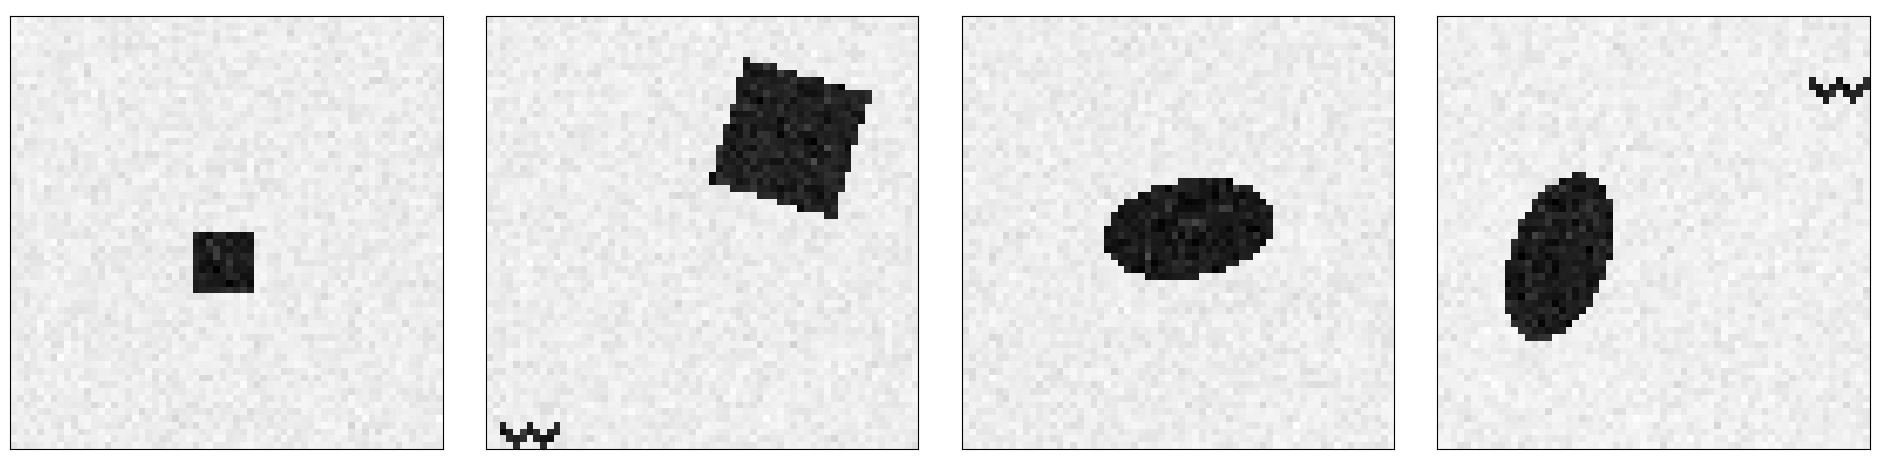
\includegraphics[width=0.4\textwidth]{images/examples_datasets_2.png}
              \end{figure}
              \pause
        \item Pattern dataset, overlapping features\\
              \begin{figure}
                  \centering
                  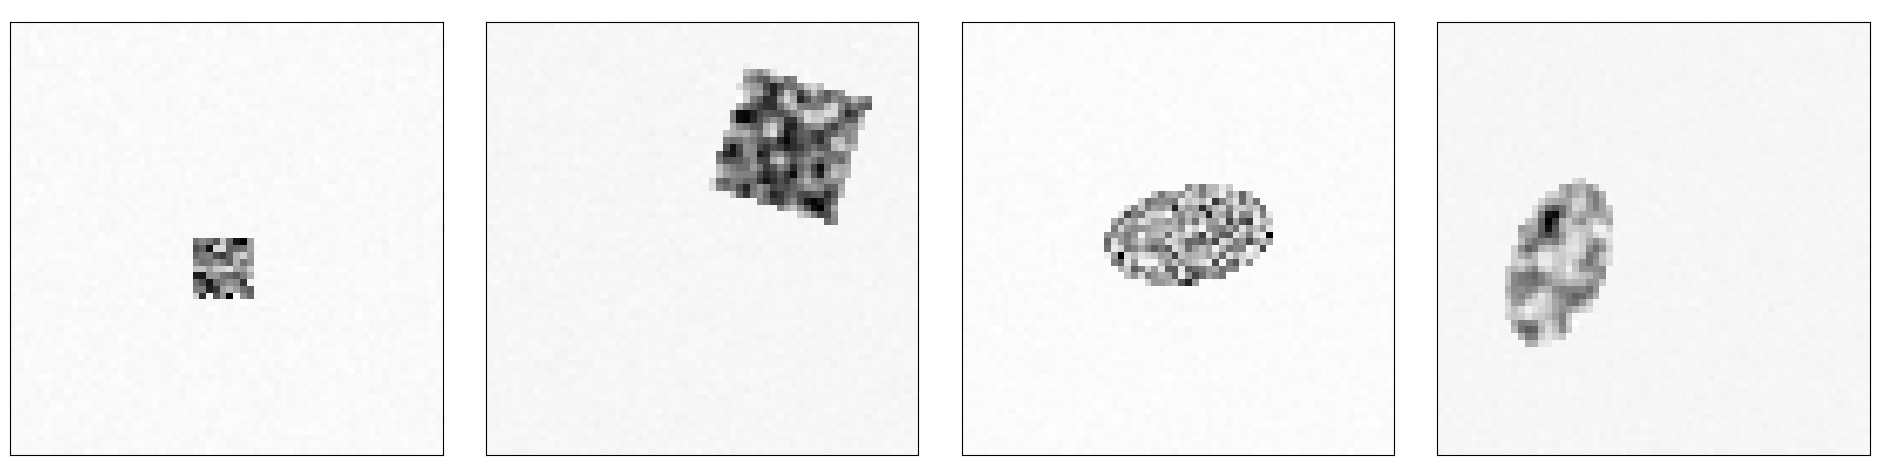
\includegraphics[width=0.4\textwidth]{images/examples_datasets_3.png}
              \end{figure}
    \end{enumerate}
\end{frame}
%----------------------------------------------------------------------------------------
\subsection{Ground Truth}
\begin{frame}[t]{Ground-Truth Feature Importance}
    Effect of Watermark $W$ on Prediction $Y$ %/ Shape $S$ on Prediction $Y$:
    \begin{align*}
        \displaystyle
        \mathrm{Watermark} & := \mathbb{E} [ Y \ | \ do(W=1) ] &  & - \mathbb{E} [ Y \ | \ do(W=0) ]
    \end{align*}
    %& \\ \mathrm{Shape}     & := \mathbb{E} [ Y \ | \ do(S=1) ] &  & - \mathbb{E} [ Y \ | \ do(S=0) ] &
    \begin{figure}[t!]
        \centering
        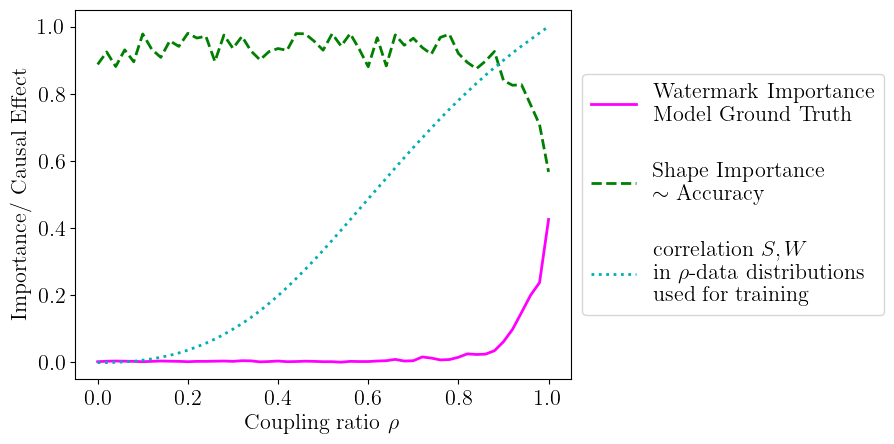
\includegraphics[width=0.7\textwidth]{images/ground_truth.png}
        \label{fig:m0_m1}
    \end{figure}
\end{frame}

%----------------------------------------------------------------------------------------
\subsection{Measures}
\begin{frame}[t]{Measures}
    Causal Effect of Intervention to Spurious Feature on Explanation: \\

    Explanation Importance $:= \mathbb{E} [ E \ | \ do(W=1) ]- \mathbb{E} [ E \ | \ do(W=0) ]$\\
    \vspace{0.5cm}
    \begin{columns}[t]
        \begin{column}[t]{.3\textwidth}
            \vspace{-0.5cm}
            \begin{figure}[t]
                $do(W=1)$ \hspace{0.13cm} $do(W=0)$
                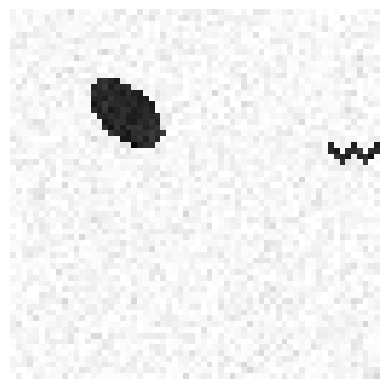
\includegraphics[width=0.45\textwidth]{images/example_image.png}
                
\includegraphics[width=0.45\textwidth]{images/example_image_false.png}
                \label{fig:example_image}
            \end{figure}
        \end{column}
        \begin{column}{.7\textwidth}
            In total 8 different metrics for measuring relative spurious feature importance in concept-based CRP explanations:
            \begin{enumerate}
                \item Direct Measures
                \item Ground-Truth-Region Measures
                \item Reference Set Measures
            \end{enumerate}
        \end{column}
    \end{columns}

\end{frame}
%----------------------------------------------------------------------------------------
\subsection{Direct Per-Concept Measures}
\begin{frame}[t]{Direct Per-Concept Measures}
    \textbf{ 1. Pixel-Wise Attribution Maps' Difference ($\AMD$)}
    \vspace{-0.4cm}
    \begin{figure}[t!]
        \centering
        concept 0 \hspace{2.5cm} concept 1 \hspace{3.7cm} concept 7\\
        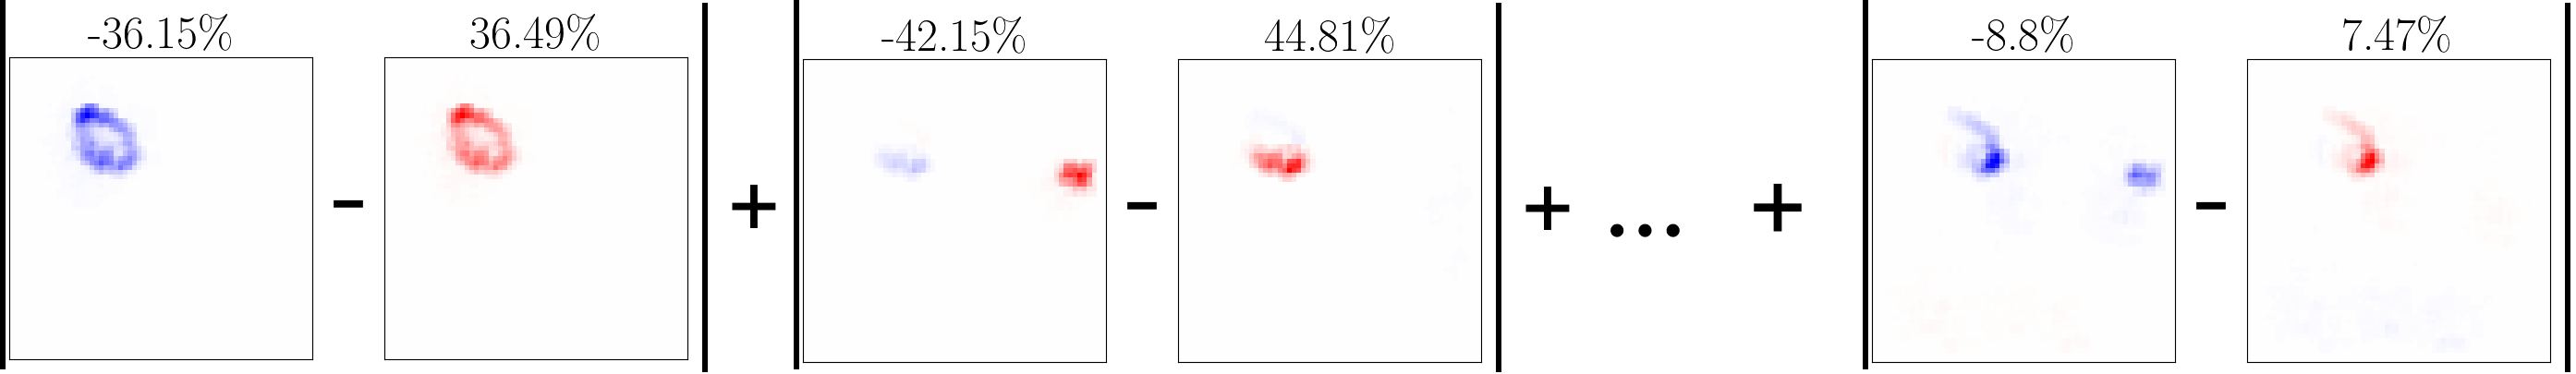
\includegraphics[width=\textwidth]{images/attr_map_diff.png}
        \label{fig:attr_map_diff}
    \end{figure}
    (2. Aggregated Relevance Vectors' Difference ($\RVD$))
    %\vspace{-0.4cm}
    %\begin{figure}[t!]
    %    \centering
    %    
\includegraphics[width=\textwidth]{images/relevance_diff.png}
    %    \label{fig:relevance_diff}
    %\end{figure}
\end{frame}
%----------------------------------------------------------------------------------------

\subsection{Region-Specific Measures}
\begin{frame}[t]{Ground-Truth-Region Measures}
    \textbf{1. Relevance Mass Accurracy ($\RMA$ \cite{Arras2022} \footpartcite{Arras2022})} \\
    Difference of importance inside bounding box
    \vspace{-0.4cm}
    \begin{figure}
        \centering
        concept 0 \hspace{2.5cm} concept 1 \hspace{3.7cm} concept 7\\
        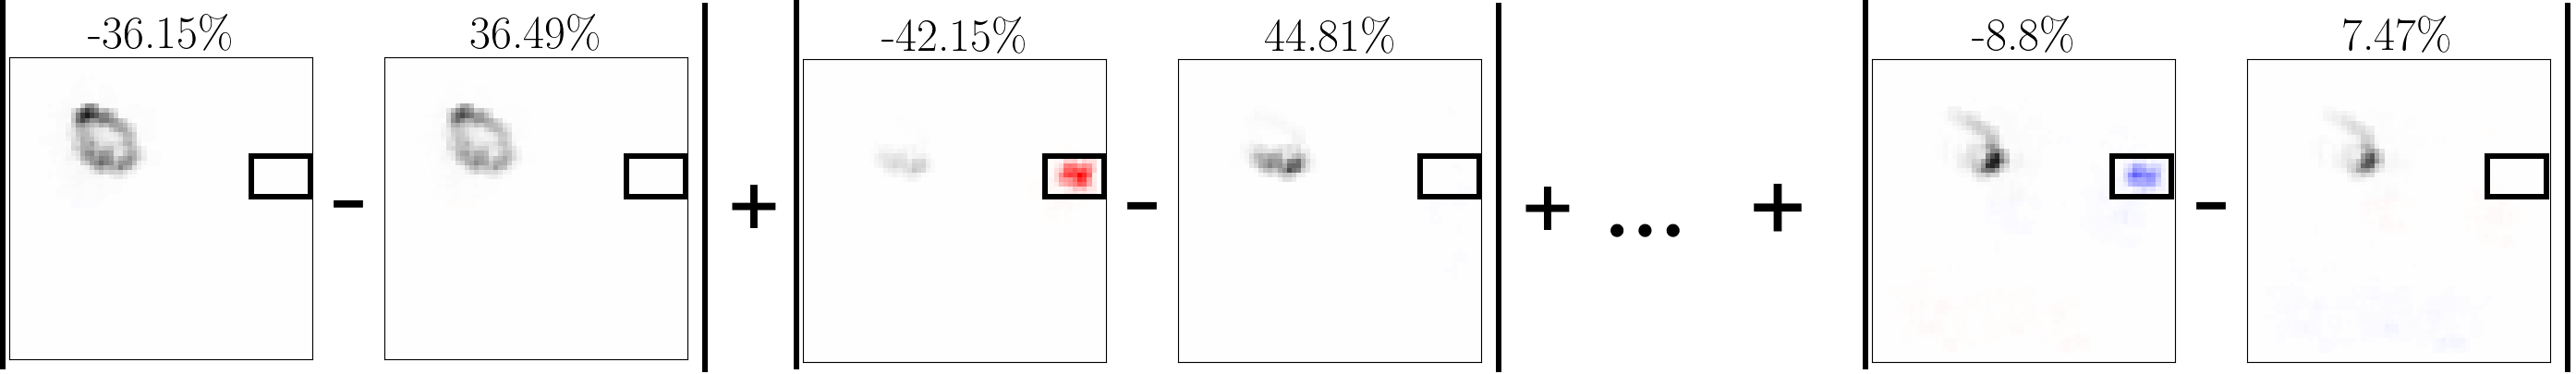
\includegraphics[width=\textwidth]{images/bbox_diff.png}
        \label{fig:bbox_diff}
    \end{figure}
    %\vspace{-0.7cm}
    (2. Relevance Rank Accuracy ($\RRA$))\\
    %Difference of number of top-k pixels in bounding box
    %\vspace{-0.4cm}
    %\begin{figure}
    %    \centering
    %    
\includegraphics[width=\textwidth]{images/rra_diff.png}
    %    \label{fig:rra_diff}
    %\end{figure}
    %\vspace{-0.7cm}
    (3. Pointing Game ($\PG$))
    %\vspace{-0.4cm}
    %\begin{figure}
    %    \centering
    %    
\includegraphics[width=\textwidth]{images/pointing_game_diff.png}
    %    \label{fig:pointing_game_diff}
    %\end{figure}
\end{frame}
%----------------------------------------------------------------------------------------

\subsection{Reference Set Measures}
\begin{frame}[t]{Reference Set Measures}
    \textbf{1. Total Relevance within most important concept's reference sets:}
    Difference of share of reference instances showing spurious feature
    (e.g. having watermark or blurry pattern)
    \vspace{-0.3cm}
    \begin{figure}[t!]
        \centering
        top concept for do(W=1) \hspace{3.3cm} top concept for do(W=0) \\
        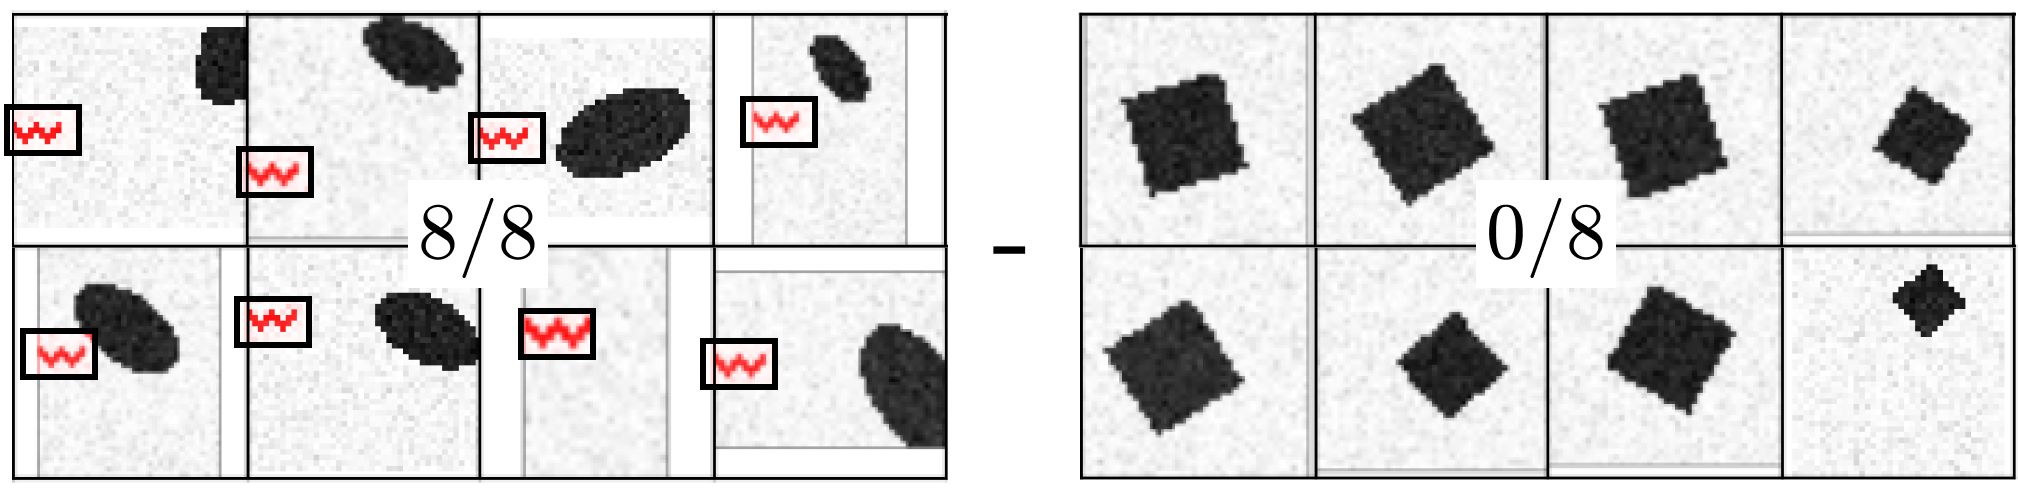
\includegraphics[width=\textwidth]{images/reference_set_diff.png}
    \end{figure}
    \vspace{-0.2cm}
    (2. In relation to images sharing core feature)\\
    (3. In class-specific reference sets)

\end{frame}
%----------------------------------------------------------------------------------------

\section[Experimental Results]{Experimental Results}

\begin{frame}[t]{Ground Truth Importance Results}
    \begin{columns}
        \begin{column}[t]{0.3\textwidth}
            \vspace{-0.8cm}
            \begin{figure}[t]
                \centering
                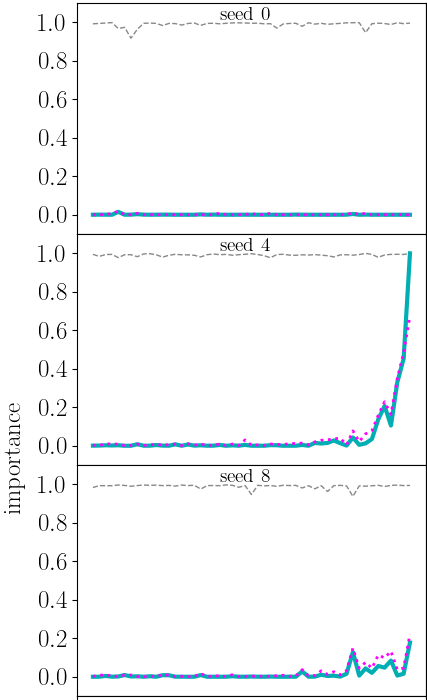
\includegraphics[width=\textwidth]{images/compare_seeds_mac_1.png}\\
                \vspace{-.3cm}
                $\rho$
            \end{figure}
        \end{column}
        \begin{column}[t]{0.38\textwidth}
            \centering
            \vspace{1cm} \\
            16 seeds $\times$ 51 vals of $\rho$ = 816 models per scenario

            $\leftarrow$ Watermark  \\

            Pattern $\rightarrow$\\
            \vspace{0.5cm}
            \begin{figure}
                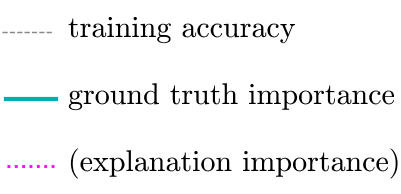
\includegraphics[width=\textwidth]{images/compare_seeds_mac_legend.png}
            \end{figure}
        \end{column}
        \begin{column}[t]{0.3\textwidth}
            \vspace{-.8cm}
            \begin{figure}[t]
                \centering
                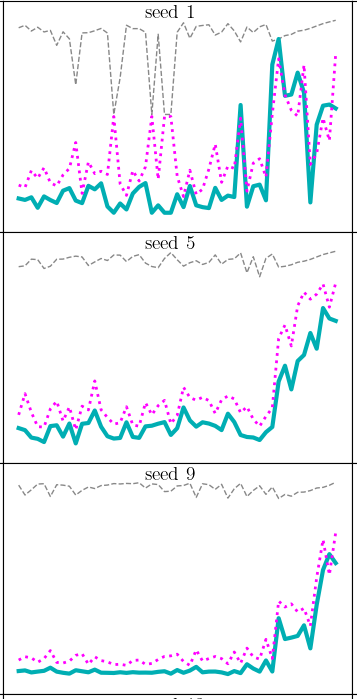
\includegraphics[width=0.84\textwidth]{images/compare_seeds_mac_2.png}\\
                \vspace{-.3cm}
                $\rho$
            \end{figure}
        \end{column}
    \end{columns}
\end{frame}
%----------------------------------------------------------------------------------------
\subsection{Comparing Results}
\begin{frame}[t]{Comparing Results}
    \begin{center}
        Watermark Scenario \hspace{3.5cm}  Pattern Scenario
    \end{center}
    \begin{figure}[t!]
        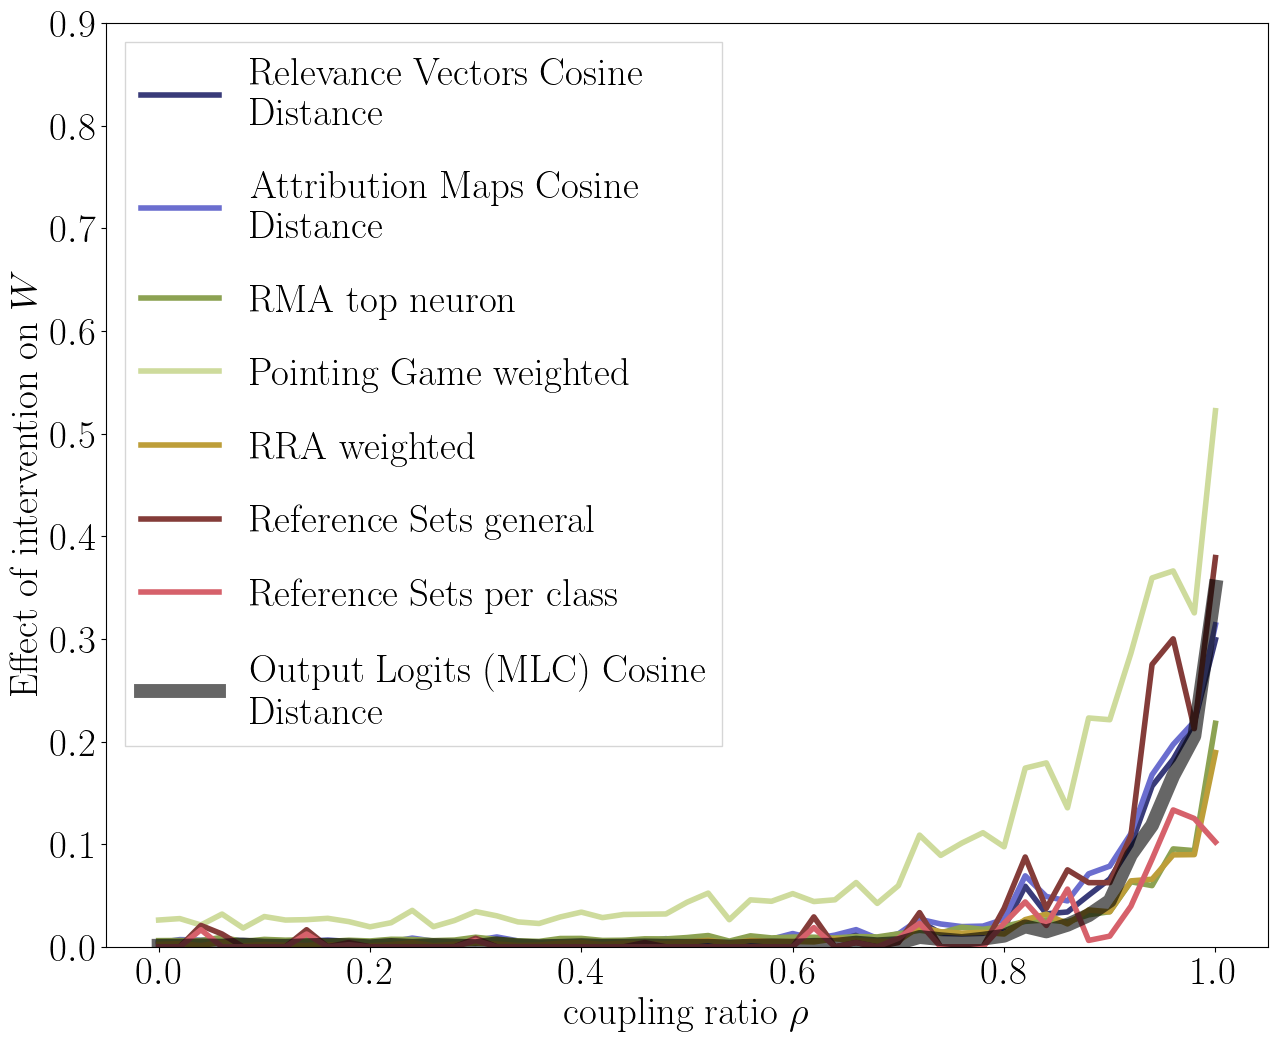
\includegraphics[width=0.49\textwidth]{images/all_results_watermark.png}
        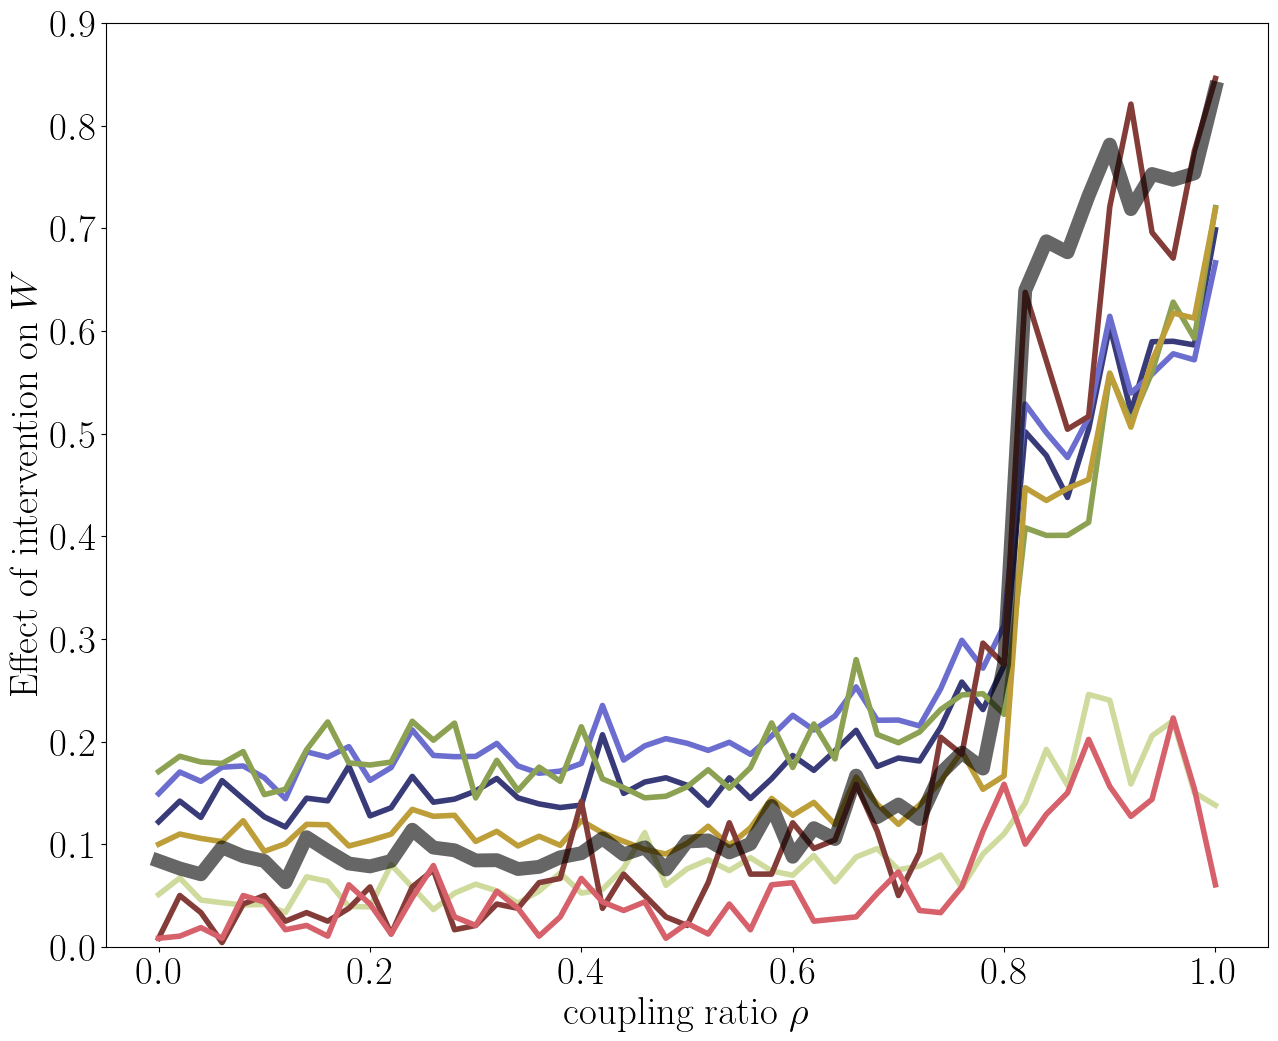
\includegraphics[width=0.49\textwidth]{images/all_results.png}
    \end{figure}
\end{frame}

%----------------------------------------------------------------------------------------

\begin{frame}[t,noframenumbering]{Comparing Results - Interpretable Relevance?}
    Examples of heatmaps for highly biased models.\\
    watermark: relevance change in- and outside of watermark region
    \begin{figure}[t!]
        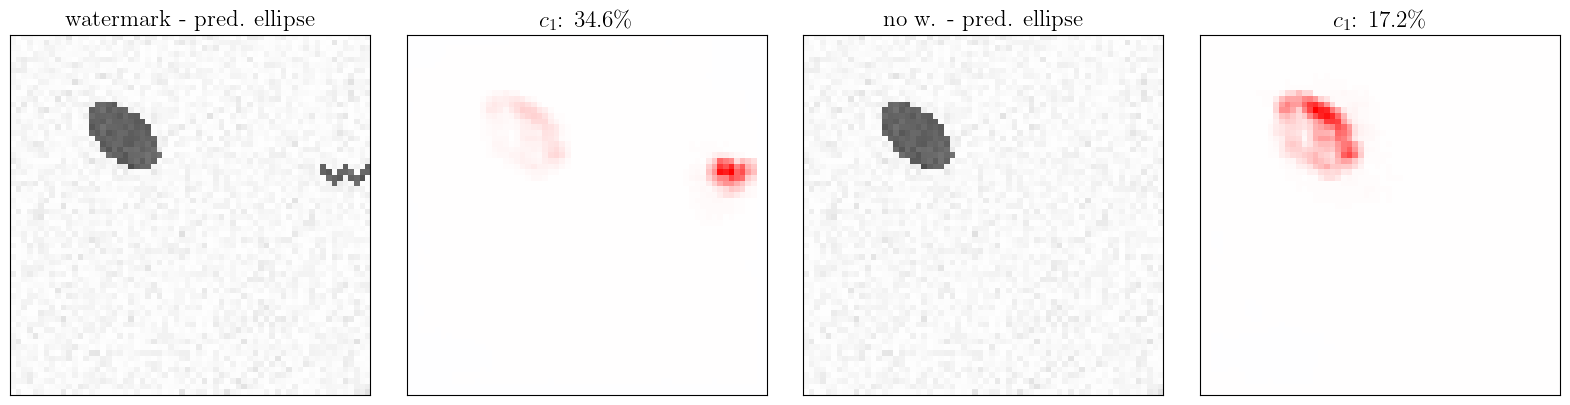
\includegraphics[width=0.6\textwidth]{images/example_relchange_outside_wm.png}
    \end{figure}
    pattern: ``shape-like'' similar heatmaps for different patterns and neurons
    \begin{figure}[t!]
        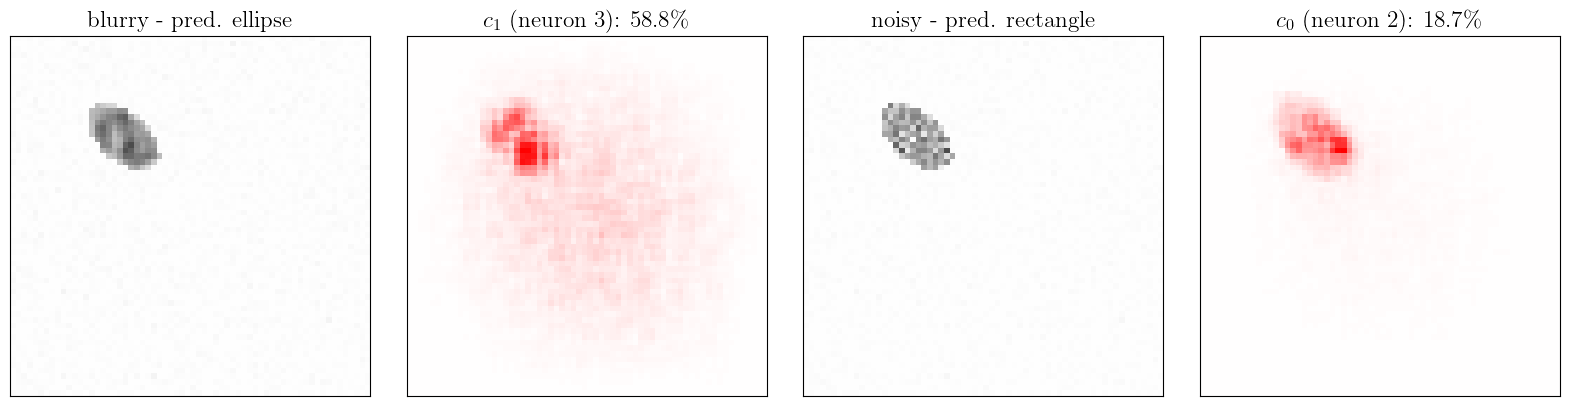
\includegraphics[width=0.6\textwidth]{images/example_top_neuron_broken.png}
    \end{figure}
\end{frame}
%----------------------------------------------------------------------------------------
\begin{frame}<1>[t, label=comparison]{Comparing Results}
    \begin{columns}
        \begin{column}[t]{0.3\textwidth}
            \begin{figure}[t!]
                \centering
                \vspace{-0.8cm}
                \begin{tikzpicture}
                    \tikzset{%
                        arrows={[scale=1.5]}
                    }
                    \node [anchor=south west,inner sep=0]  (wm) at (0,0) {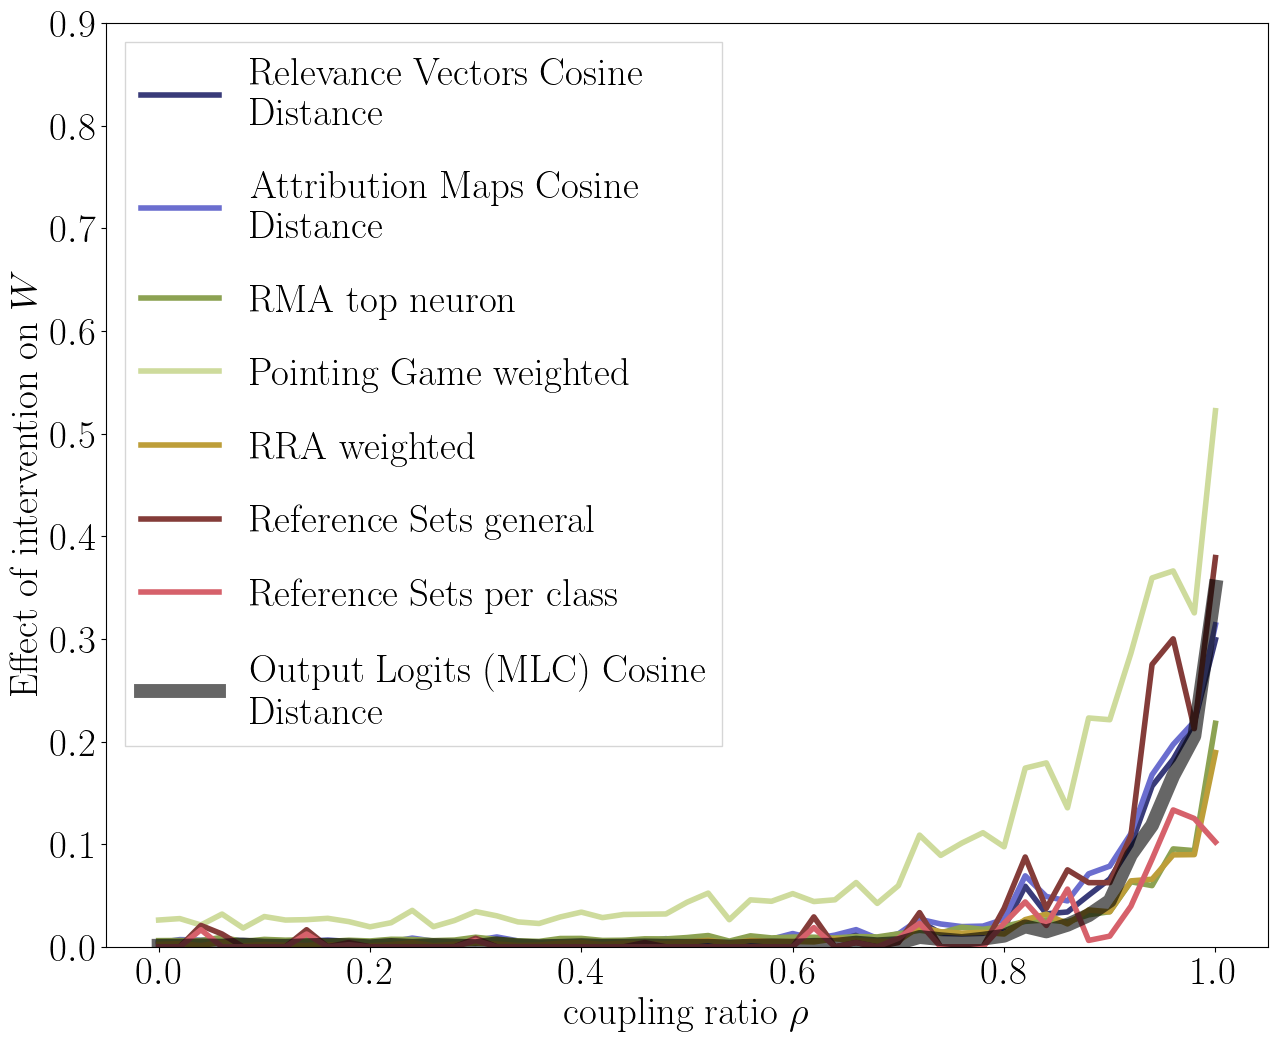
\includegraphics[width=\textwidth]{images/all_results_watermark.png}};
                    \only<2>{\draw[->, draw=teal] (4.0, 0.4) -- (3.9,0.7);}
                \end{tikzpicture}
                \begin{tikzpicture}
                    \node [anchor=south west,inner sep=0]  (pa) at (0,0) {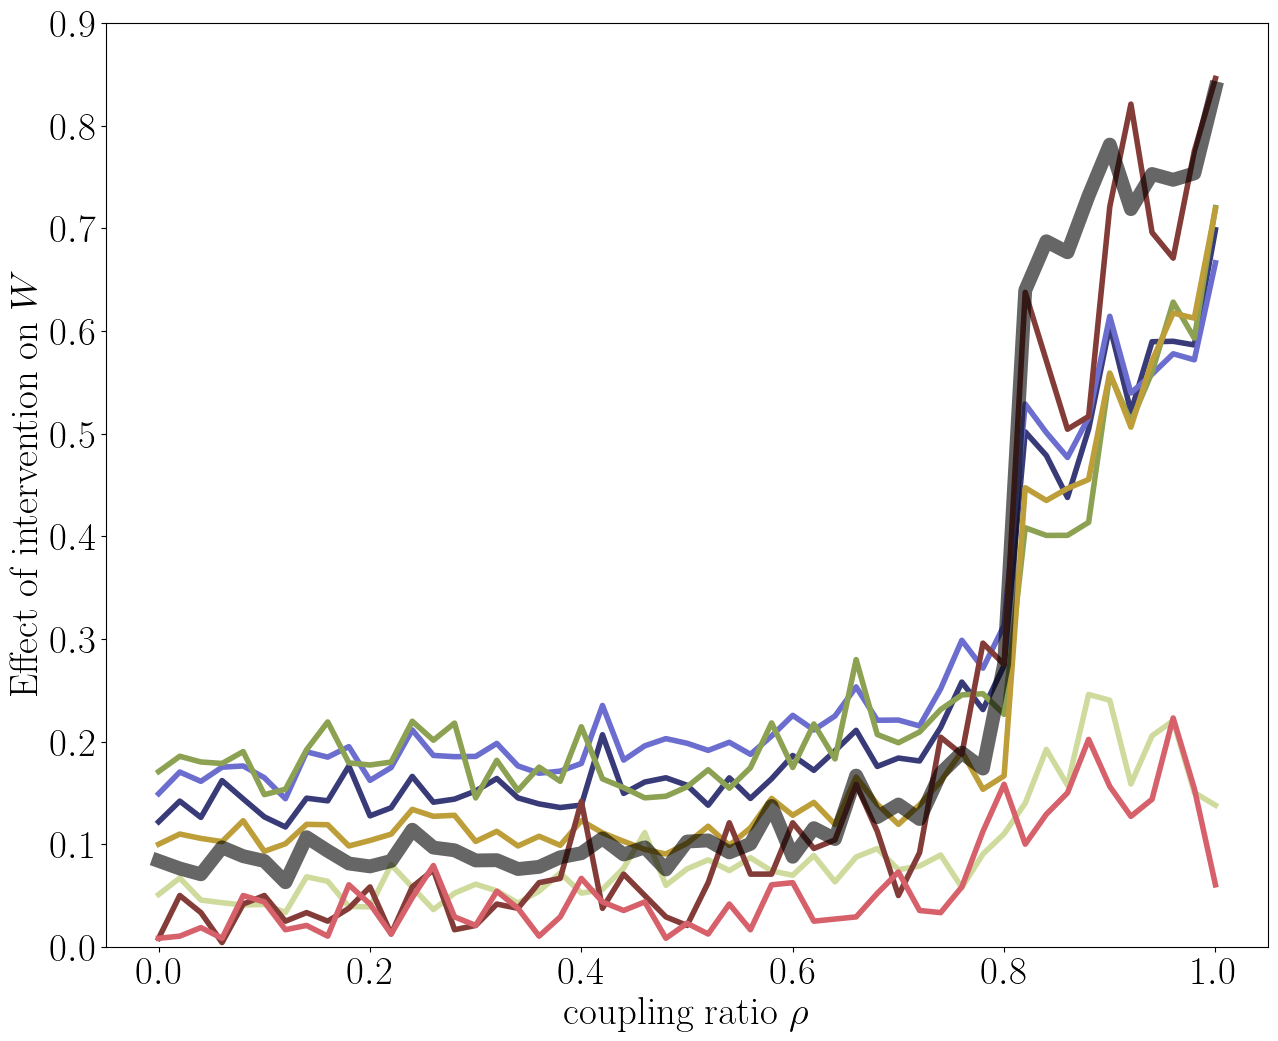
\includegraphics[width=\textwidth]{images/all_results.png}};
                    \only<2>{\draw[->, draw=teal] (4.0, 0.6) -- (3.7,0.8);}
                    \only<1>{\draw[->, draw=teal] (4.0, 1.7) -- (3.9,2.2);}
                \end{tikzpicture}
            \end{figure}
        \end{column}
        \begin{column}[t]{0.6\textwidth}
            \begin{itemize}
                \item Especially watermark scenario: follows ground truth
                \item Pattern Scenario: overlapping features interfer with explanation effect \pause
                \item Class-specific reference set measure fails due to entanglement
            \end{itemize}
        \end{column}
    \end{columns}
\end{frame}

\begin{frame}[t,noframenumbering]{Comparing Results - Entanglement}
    Core and spurious feature are not disentangled by individual neurons\\
    $\rightarrow$ Reference sets encode shape together with watermark/texture
    \begin{figure}[ht!]
        \centering
        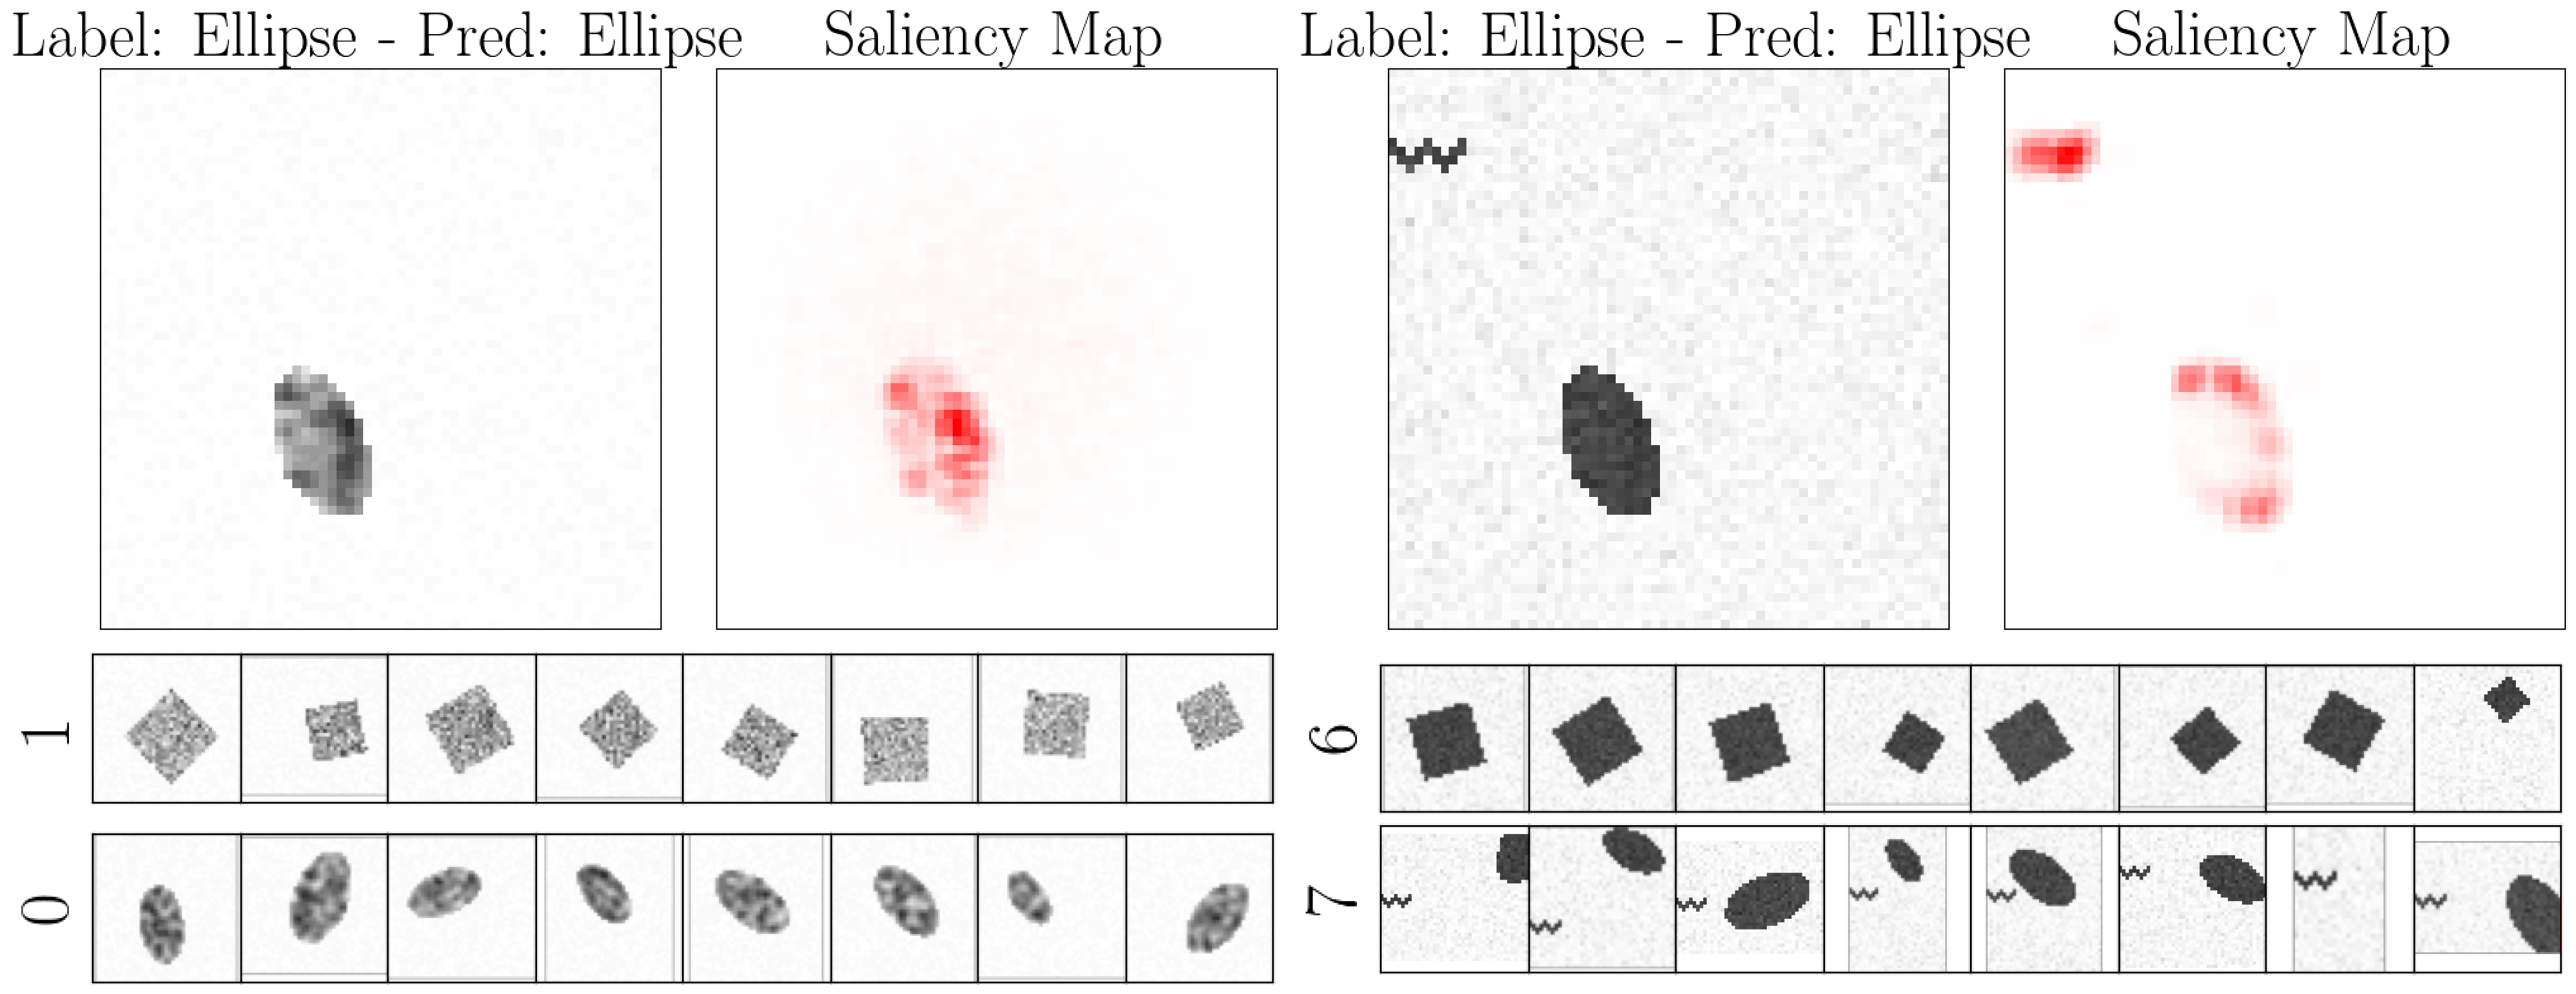
\includegraphics[width=\textwidth]{images/no_disentanglement.png}
        \label{fig:no_disentanglement}
    \end{figure}
\end{frame}
\againframe<2>[noframenumbering]{comparison}

%----------------------------------------------------------------------------------------
\section[Conclusion and Outlook]{Conclusion and Outlook}
\begin{frame}{Conclusion}
    \textbf{Main Result:} Explained relative spurious feature importance is close to model ground-truth and not data distribution

    but:

    \begin{itemize}
        \item Entanglement of core/spurious feature in explanation can produce misleading scores
        \item Lacking consensus for ``good'' explanation complicates quantitative evaluation
        \item Trade-off: high fidelity - human interpretability or complexity of explanation
    \end{itemize}
\end{frame}
%----------------------------------------------------------------------------------------
\begin{frame}
    \frametitle{Outlook}
    \begin{itemize}
        \item More complex problems
        \item Comparison to other concept-based methods or pure LRP
        \item Other causal models of data generation
    \end{itemize}
    \begin{figure}[t!]
        \centering
        \tikzset{%
            neuron/.style={
                    ellipse,
                    draw,minimum width=6mm,
                    minimum height=6mm,inner sep=1pt
                },
        }
        \begin{tikzpicture}[scale=0.7]
            \node [neuron]  (nw) at (0,2) {$\mathcal{N}_W$};
            \node [neuron]  (ns) at (0,0) {$\mathcal{N}_S$};
            \node [neuron]  (w) at (2,2) {$W$};
            \node [neuron]  (s) at (2,0) {$S$};
            \node [neuron, inner sep=0pt]  (i) at (4,1) {Image};
            \node [draw, inner sep=6pt]  (ibox) at (4,1) {Image};
            \node []  (ibox) at (4,2) {selection};

            \draw[->] (nw) -- (w);
            \draw[->] (ns) -- (s);
            \draw[->] (w) -- (i);
            \draw[->] (s) -- (i);
        \end{tikzpicture}
    \end{figure}
\end{frame}
%------------------------------------------------

\begin{frame}[allowframebreaks,noframenumbering]
    \frametitle{References}
    \printbibliography
    %\bibliographystyle{plain}
    %\bibliography{bibdata.bib}
    Code of experiments:\\ \url{https://github.com/lillijo/xai-evaluation-master-thesis}

\end{frame}

%------------------------------------------------
\begin{frame}[noframenumbering]
    Different Structural Causal Models producing the same distribution
    \begin{figure}[t!]
        \centering
        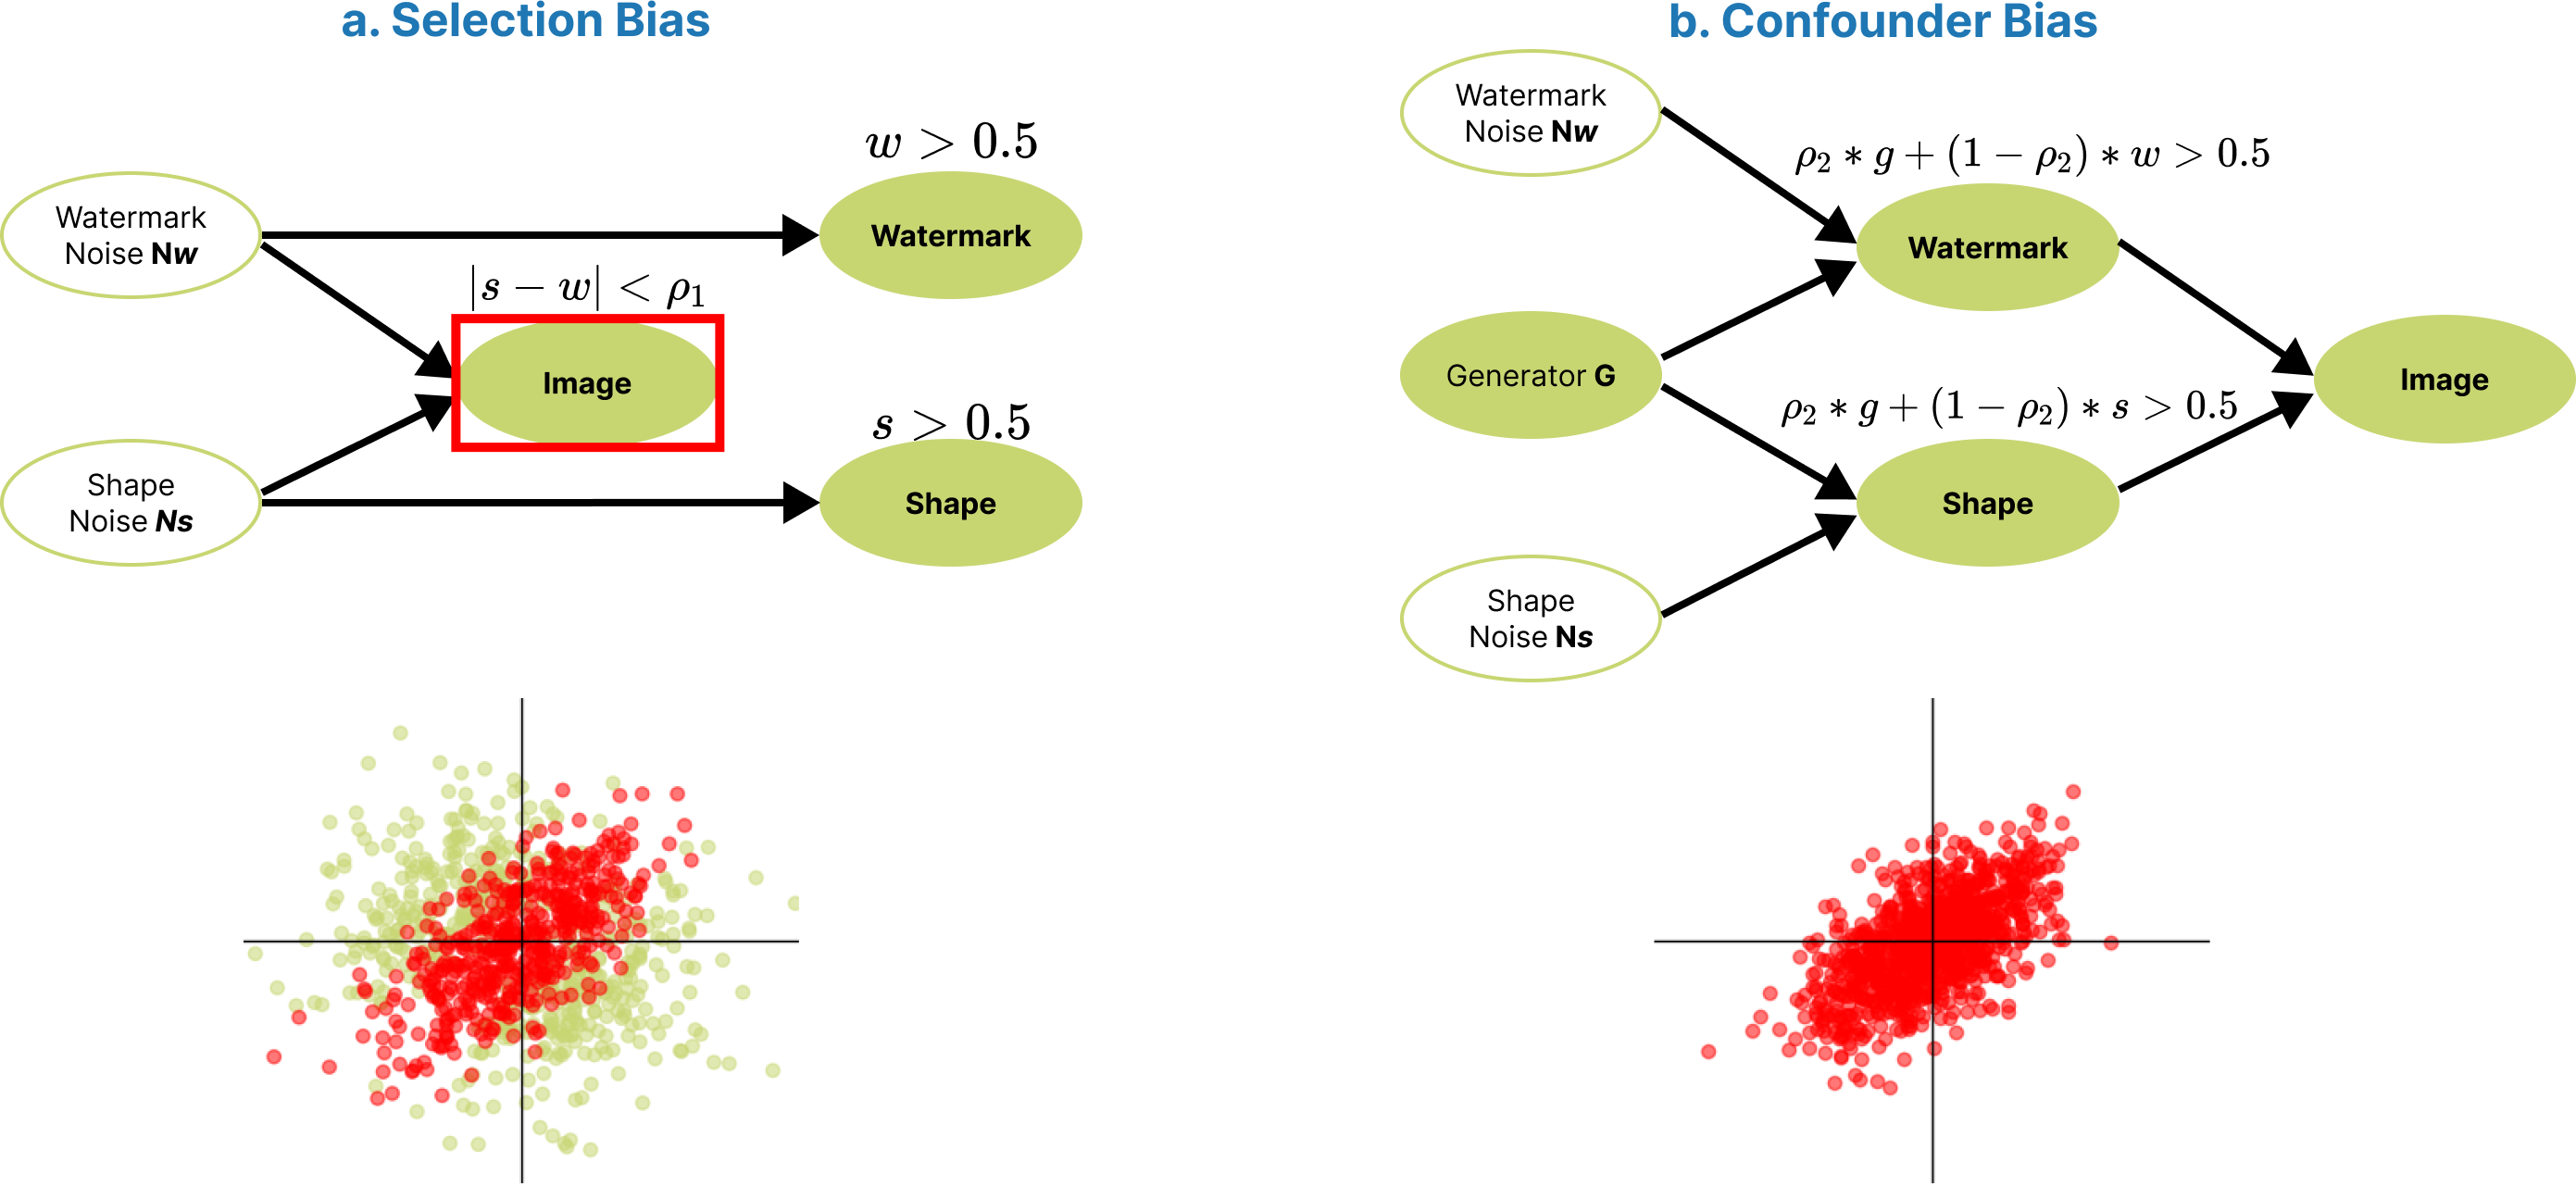
\includegraphics[width=\textwidth]{images/equivalent_scm.png}
        \label{fig:equivalent_scm}
    \end{figure}
\end{frame}
%------------------------------------------------
\begin{frame}[noframenumbering]
    Full set of concept-conditional attribution maps
    \begin{figure}[t!]
        \centering
        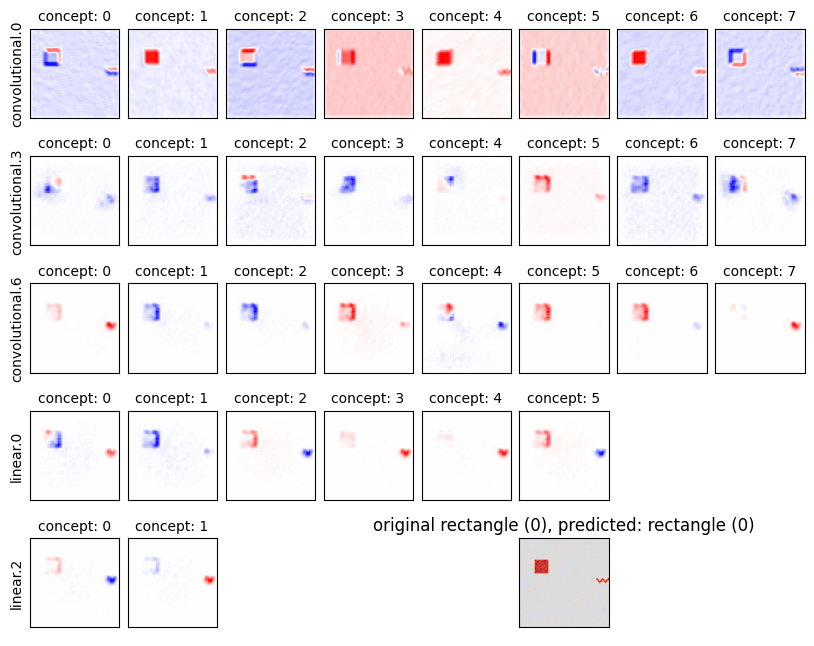
\includegraphics[width=0.9\textwidth]{images/conditional_heatmaps.png}
        \label{fig:conditional_heatmaps}
    \end{figure}
\end{frame}

%------------------------------------------------
\begin{frame}[noframenumbering]
    Full set of concept-conditional attribution maps for pattern dataset
    \begin{figure}[t!]
        \centering
        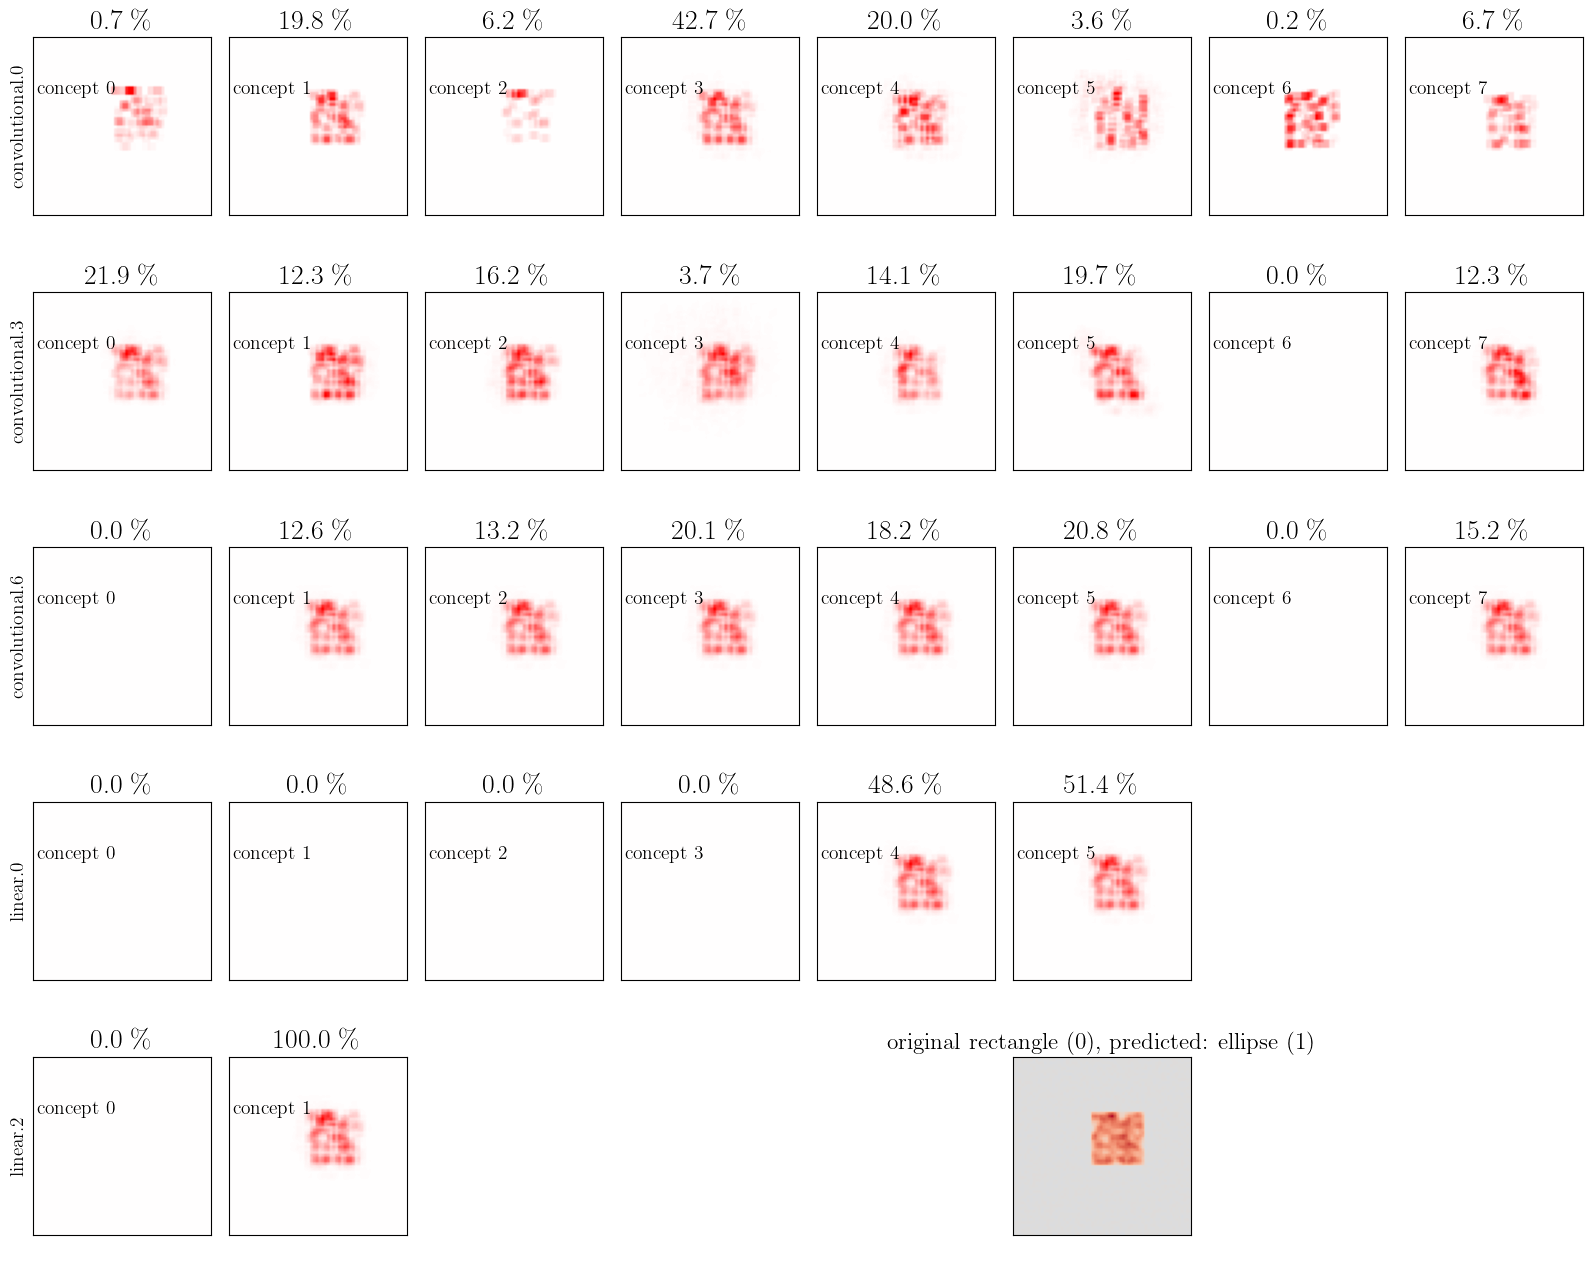
\includegraphics[width=0.9\textwidth]{images/attributions_pattern2.png}
        \label{fig:attributions_pattern2}
    \end{figure}
\end{frame}
%------------------------------------------------
\begin{frame}[noframenumbering]
    Feature Importance over $\rho$ for all generating factors
    \begin{figure}[t!]
        \centering
        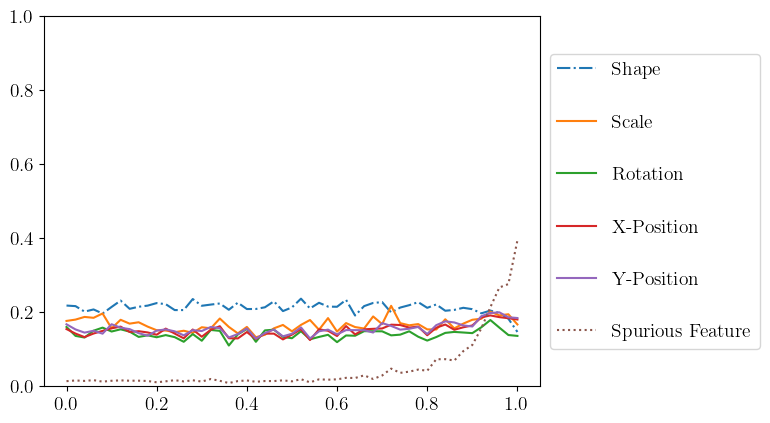
\includegraphics[width=0.49\textwidth]{images/relevance_all_factors.png}
        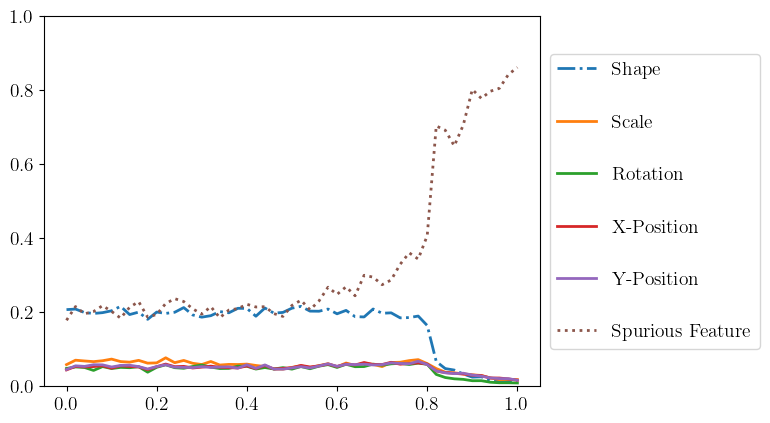
\includegraphics[width=0.49\textwidth]{images/relevance_all_factors_overlap.png}
        \label{fig:relevance_all_factors}
    \end{figure}
\end{frame}
%------------------------------------------------
\begin{frame}[noframenumbering]
    Ground Truth and attributed importance over all seeds (watermark scenario)
    \begin{figure}[t!]
        \centering
        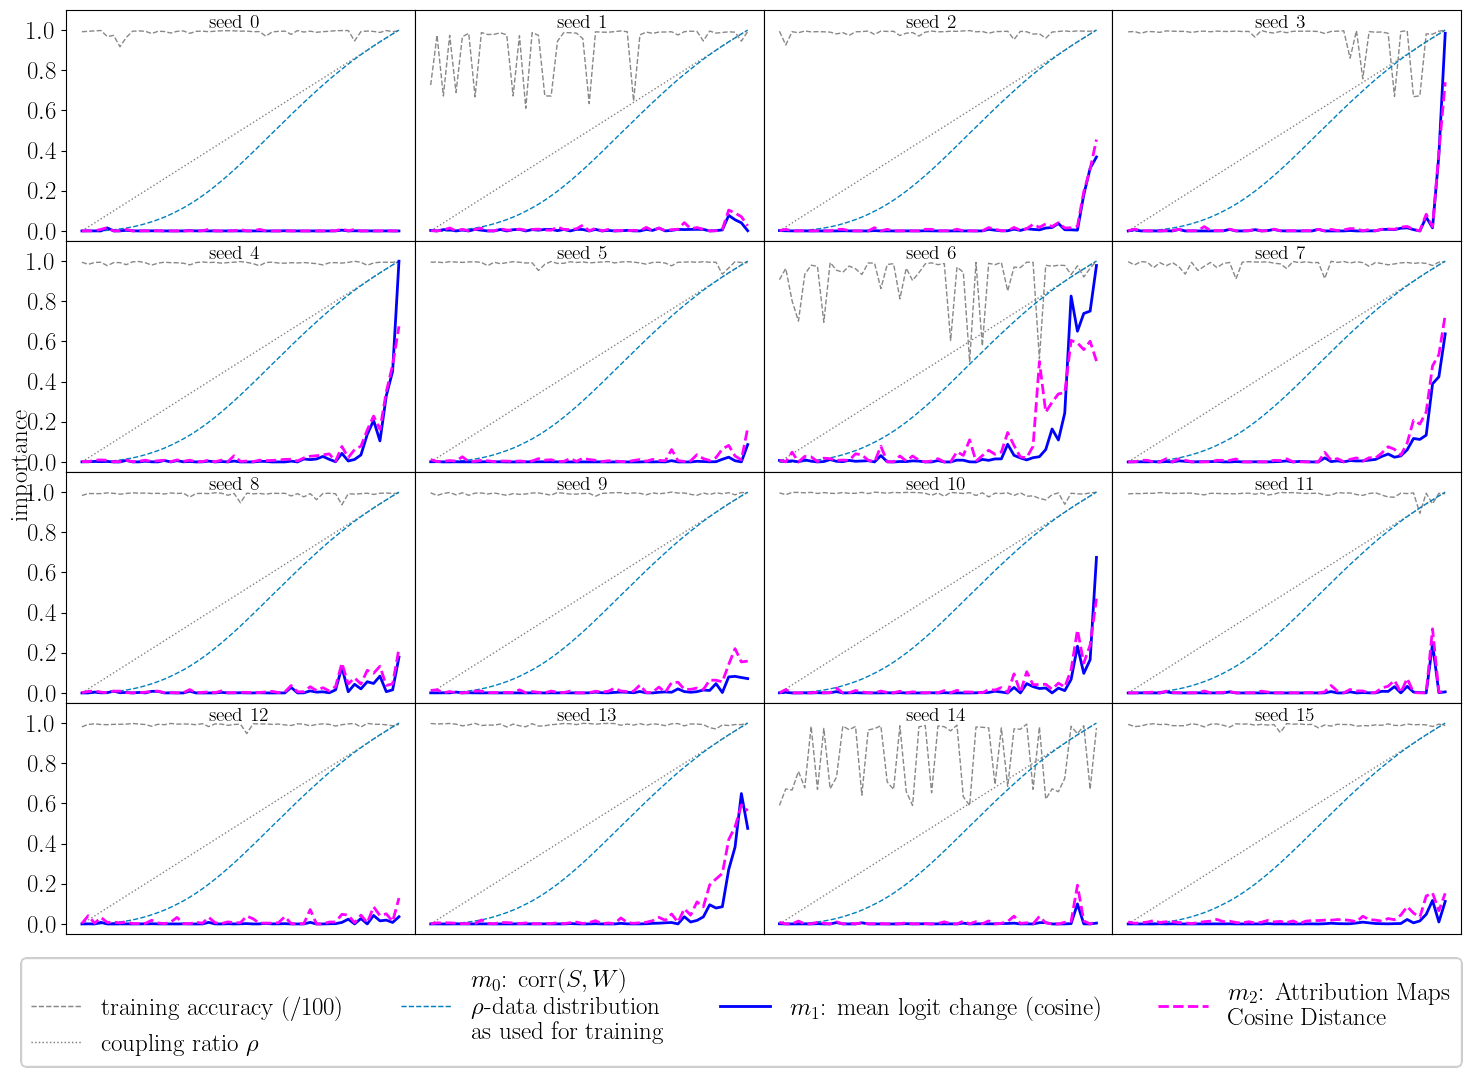
\includegraphics[width=0.9\textwidth]{images/compare_seeds_mac.png}
        \label{fig:compare_seeds_mac}
    \end{figure}
\end{frame}
%------------------------------------------------
\begin{frame}[noframenumbering]
    Ground Truth and attributed importance over all seeds (pattern scenario)
    \begin{figure}[t!]
        \centering
        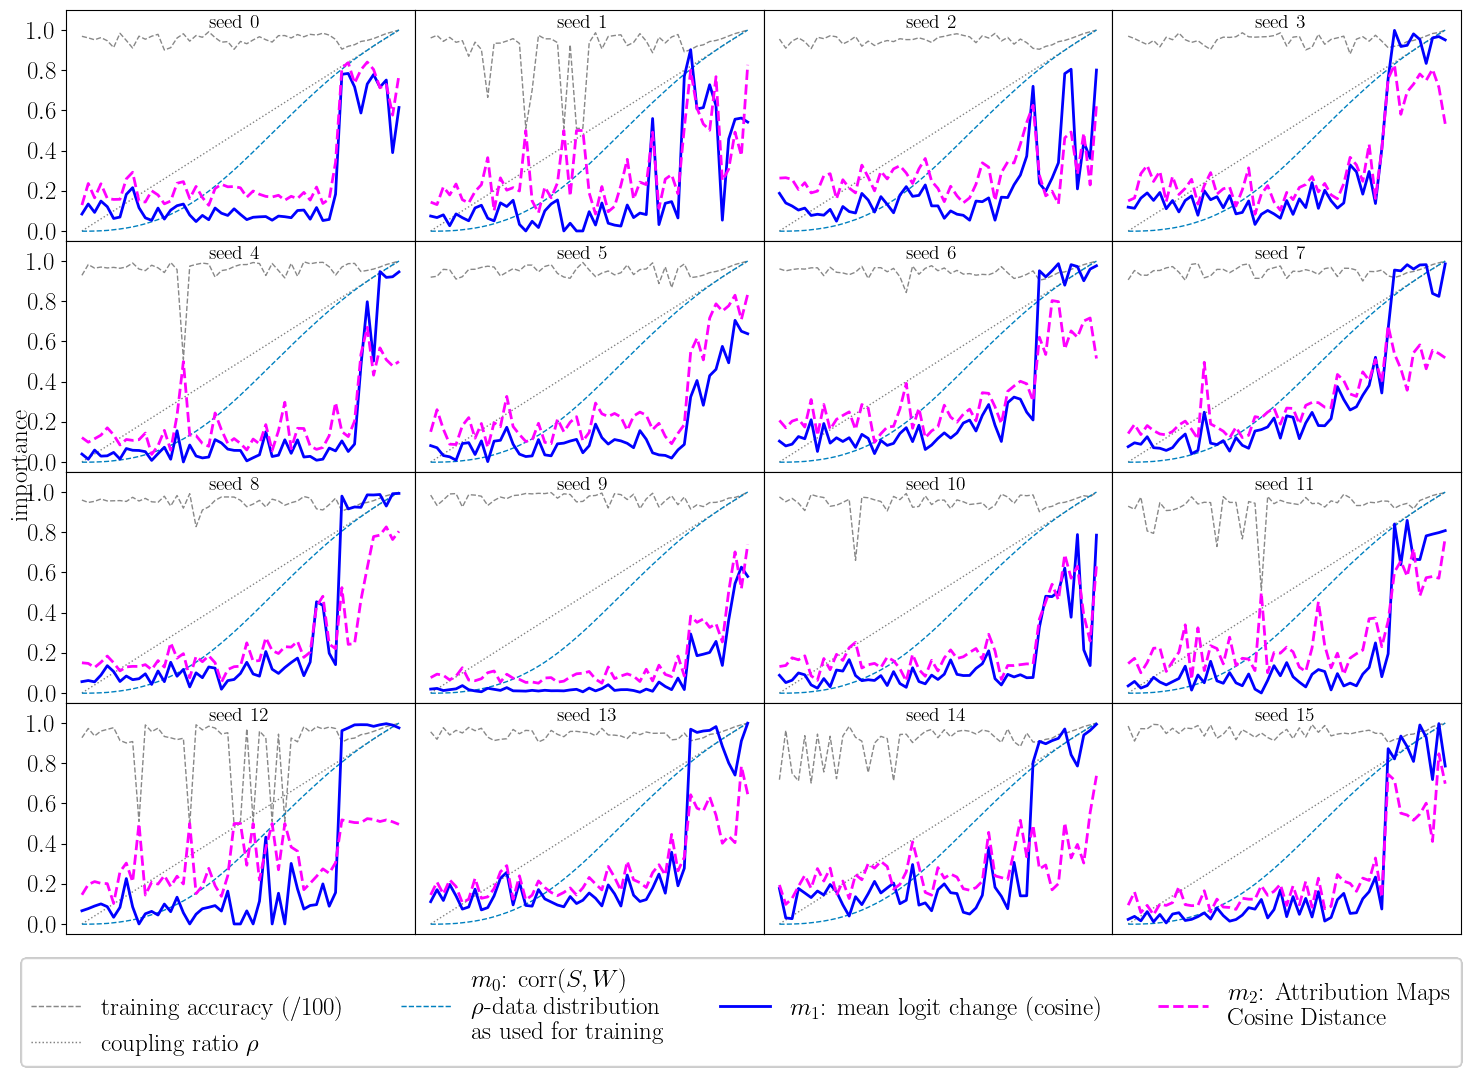
\includegraphics[width=0.9\textwidth]{images/compare_seeds_overlap.png}
        \label{fig:compare_seeds_overlap}
    \end{figure}
\end{frame}

\end{document}